%%%Pour afficher les réponses , activer l'option "answers" de la ligne documentclass
%Sans réponses
%\documentclass[twoside,a4paper,11pt]{exam}
%avec réponses
\documentclass[twoside,a4paper,11pt,answers]{exam}


\title{XX 1}
\date{}
\author{Juliette Fenogli}


\usepackage{siunitx}
\usepackage{mystyles}
\usepackage[export]{adjustbox}
\usepackage{mathpazo}
\usepackage{booktabs}
\usepackage{framed}
\usepackage{listings}
\usepackage{mhchem}



\lstset
{upquote=true,
columns=flexible,
    basicstyle=\small\tt\hbox{}, 
	basicstyle=\ttfamily,
	language=Python,
    framesep=\fboxsep,
    framerule=\fboxrule,
    xleftmargin=\dimexpr\fboxsep+\fboxrule,
    xrightmargin=\dimexpr\fboxsep+\fboxrule,
	commentstyle=\color{gray},
	frame=single,
	rulecolor=\color{green!5},
	backgroundcolor=\color{gray!5},
	breaklines,
	numbers=left, 
	numbersep=5pt,  
	numberstyle=\scriptsize \ttfamily\color{gray},
	breakindent=1.5em,
	literate={Δ}{{$\mathtt{\Delta}$}}1 {‡}{{$\mathtt{\ddagger}$}}1
  {á}{{\'a}}1 {é}{{\'e}}1 {í}{{\'i}}1 {ó}{{\'o}}1 {ú}{{\'u}}1
  {Á}{{\'A}}1 {É}{{\'E}}1 {Í}{{\'I}}1 {Ó}{{\'O}}1 {Ú}{{\'U}}1
  {à}{{\`a~}}1 {è}{{\`e}}1 {ì}{{\`i}}1 {ò}{{\`o}}1 {ù}{{\`u}}1
  {À}{{\`A~}}1 {È}{{\'E}}1 {Ì}{{\`I}}1 {Ò}{{\`O}}1 {Ù}{{\`U}}1
  {ä}{{\"a}}1 {ë}{{\"e}}1 {ï}{{\"i}}1 {ö}{{\"o}}1 {ü}{{\"u}}1
  {Ä}{{\"A}}1 {Ë}{{\"E}}1 {Ï}{{\"I}}1 {Ö}{{\"O}}1 {Ü}{{\"U}}1
  {â}{{\^a}}1 {ê}{{\^e}}1 {î}{{\^i}}1 {ô}{{\^o}}1 {û}{{\^u}}1
  {Â}{{\^A}}1 {Ê}{{\^E}}1 {Î}{{\^I}}1 {Ô}{{\^O}}1 {Û}{{\^U}}1
  {œ}{{\oe}}1 {Œ}{{\OE}}1 {æ}{{\ae}}1 {Æ}{{\AE}}1 {ß}{{\ss}}1
  {ç}{{\c c}}1 {Ç}{{\c C}}1 {ø}{{\o}}1 {å}{{\r a}}1 {Å}{{\r A}}1
  {€}{{\EUR}}1 {£}{{\pounds}}1 {×}{{$\times$}}1,       
}

\usepackage{adjustbox}



\begin{document}

\includepdf[pages = {1}]{page-garde.pdf}


\newpage
\tito{Molécules naturelles}



\section{Synthèse d'un composé odorant naturel : l'acétate de benzyle}

L’acétate de benzyle constitue l’odeur de tête du jasmin. Cette molécule est présente dans beaucoup de fleurs et peut aussi être obtenue par synthèse organique selon la réaction donnée figure \ref{fig:synthese}.

\begin{center}
    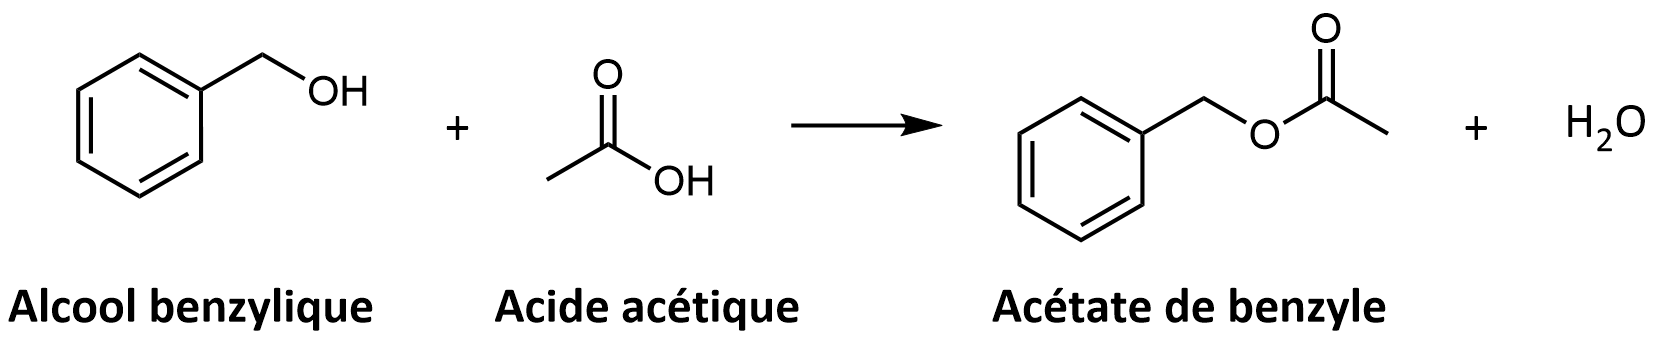
\includegraphics[scale=0.3]{images/synthese_acetate_benzyle.png}
    \captionof{figure}{Réaction de synthèse de l'acétate de benzyle}
    \label{fig:synthese}
\end{center}


\begin{questions}
\begin{framed}
\question De quel type de réaction s'agit-il ?
\begin{solution}[2cm]
Il s'agit d'une substitution sur un acide, ici plus spécifiquement une estérification de Fischer.
\end{solution}
\end{framed}

%\fullwidth{\subsection{Caractérisations}

%end fullwidth pour utiliser toute la largeur du document
%}
\paragraph*{Protocole}

~

Dans un ballon monocol de 50 mL, introduire 3 mL d’acide éthanoïque glacial, 5,2 g d’alcool benzylique et 10 mL de cyclohexane. Ajouter 100 mg d’APTS. Installer le Dean-Stark sur le col du ballon. Chauffer à reflux le mélange réactionnel pour environ 30 minutes.

\begin{solution}

\begin{tabular}{c|c|c|c|c|c|c|c}
\toprule
%    Composé & état physique & m (g) & V (mL) & M ($\unit{g.mol^{-1}}$) & d & n (mmol) & éq. \\
    \hline
     Acide acétique glacial  & liquide & 3.24 & 3 &	60.06	& 1,08	& 54	& 1,1 \\
Alcool benzylique & liquide	& 5,2	& 5	& 108,15	& 1,04 & 48 &	1 \\
APTS	& solide	& 0.1 &		& 172.21 & & 0.6 & 0.01 \\
 \bottomrule
\end{tabular}

    Il faut chauffer pas mal pour terminer en 30 minutes, en calorifugeant éventuellement le Dean-Stark avec du papier aluminium.
    Vérifier qu'ils ont bien rempli à affleurement le tube du Dean-Stark avec du cyclohexane.
\end{solution}

\begin{framed}
\question Quel est le rôle de l'APTS ?
\begin{solution}[1cm]
Il s'agit du catalyseur acide.
\end{solution}
\end{framed}

\begin{framed}
\question Comment repérer simplement si la réaction est terminée ?
\begin{solution}[2cm]
Avec la quantité d'eau contenue dans le tube du réfrigérant. On introduit ici 48 mmol d'alcool benzylique comme réactif limitant. Il faut également prendre en compte l'APTS qui est monohydraté. La quantité d'eau attendue dans le tube du Dean Stark en fin de réaction est donc de $48,6 \cdot 18 = 0,87 mL$.

\end{solution}
\end{framed}

\par Analyser le milieu réactionnel par chromatographie sur couche mince avec pour éluant un mélange cyclohexane/acétate d’éthyle : 8/2.

~

\par Ajouter 10 mL d’eau distillée puis transvaser le milieu réactionnel dans une ampoule à décanter. Séparer les phases aqueuse et organique puis extraire la phase aqueuse avec 2 $\times$ 10 mL d’éther diéthylique. Rassembler les phases organiques et les laver avec 30 mL d'une solution saturée d’hydrogénocarbonate de sodium $\ce{NaHCO3(sat)}$. Faire le mélange dans l'erlenmeyer dans un premier temps, puis laver et séparer dans l'ampoule à décanter. Laver de nouveau la phase organique avec 30 mL d'une solution saturée de chlorure de sodium $\ce{NaCl(sat)}$.
%environ 30 mL pour chaque solution, l'elève doit choisir en fonction du volume de phase organique qu'il a à laver.%{(sat.)}{(sat.)}

\begin{framed}
\question Quel est l'objectif de l'extraction liquide-liquide ? Pourquoi faire 2 extractions avec 10 mL de solvant plutôt qu'une seule extraction à 20 mL de solvant ? 
\begin{solution}[2cm]
Récupérer l'acétate de benzyle éventuellement présent en phase aqueuse. Multilier les extractions pour un même volume de solvant permet d'augmenter le rendement de l'extraction.
\end{solution}
\end{framed}

\begin{framed}
\question Quel est l'objectif du lavage à la solution de \ce{NaHCO3} saturée ? Quel est le gaz dégagé ?
\begin{solution}[2cm]
On veut neutraliser l'excès d'acide acétique et l'APTS éventuellement présent en phase organique pour les faire passer en phase aqueuse (l'ion carboxylate y est plus soluble). Le gaz dégagé est du \ce{CO2} : 
\begin{equation*}
    \ce{HCO3-} \quad + \quad \ce{CH3COOH} \quad \longrightarrow \quad \ce{CO2} \quad + \quad \ce{H2O} \quad + \quad \ce{CH3COO-}
\end{equation*}
\end{solution}
\end{framed}

Sécher la phase organique avec \ce{MgSO4}, filtrer et évaporer le solvant sous pression réduite. 
\par \textit{Demander l’aide d'un examinateur pour l’utilisation de l’évaporateur rotatif.}

\begin{framed}
    \question Proposer une méthode de caractérisation de l’huile obtenue et la mettre en œuvre. 
\begin{solution}[2cm]
     Mesure de l'indice de réfraction au réfractomètre d'Abbe. Si l'indice n'est pas le bon, c'est surement signe qu'il reste de l'alcool benzylique.
\end{solution}
\end{framed}

\begin{framed}
    \question Proposer une méthode de purification du produit obtenu. En expliquer le principe.
\begin{solution}[3cm]
     Distillation ou chromatographie sur colonne.
\end{solution}
\end{framed}

\begin{framed}
    \question Calculer le rendement de la réaction.
\begin{solution}[3cm]
     La masse molaire de l'acétate de benzyle vaut 150,18 \si{\gram\per\mol}, on s'attend donc au maximum à avoir une masse de produit obtenu égale à $ 0,048 \cdot 150,18 = 7,2 g$. Le rendement obtenu devrait être voisin de 90\%.
\end{solution}
\end{framed}


\end{questions}

\newpage

\section{Dosage du curcumin contenu dans la poudre de curcuma}

La poudre obtenue par broyage de la poudre du curcuma longa L. (plante de la famille du gingembre) est un des principaux ingrédients du curry. Cette racine possède des propriétés anti-oxydantes, notamment grâce aux curcuminoïdes qu'elle contient. Ces composés dérivent de la molécule de curcumin représentée figure \ref{fig:curcumin}, qui est aussi responsable de la couleur jaune intense du curcuma. L'objectif de cette partie est de doser la quantité de curcumin effectivement présente dans une poudre de curcuma commerciale (environ 3\% d'après les indications de l'étiquette).

\begin{center}
    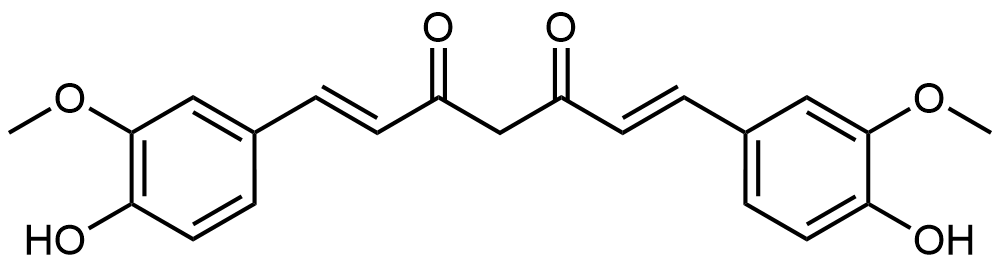
\includegraphics[scale=0.3]{images/curcumin.png}
    \captionof{figure}{Curcumin}
    \label{fig:curcumin}
\end{center}

On dispose d'une solution de curcumin dans l'éthanol de concentration massique 1,0 %$\unit{g.L^{-1}}$
(\textbf{solution A}).


\paragraph{Protocole}

~

\par Dans une fiole jaugée de 100 mL contenant 1 mL d'acide acétique glacial, diluer 100 fois la solution A dans l'éthanol. On obtient alors la \textbf{solution B}.

\begin{solution}
    Prélèvement de 1 mL à la pipette jaugée de A à diluer dans la fiole de 100 mL.
\end{solution}

~

\par Réaliser une gamme de solutions étalons de concentrations massiques comprises entre $1.10^{-3}$ et $1.10^{-2}$ %\unit{g.L^{-1}}.

\begin{solution} 

On dispose de 4 fioles jaugées de 10 mL. Il suffit alors de diluer quelques mL de la solution B dans l'éthanol.

~

 \begin{center}
     
\begin{tabular}{c|c}
\centering
%     Volume prélevé de solution B (mL) & Concentration massique (\unit{g.L^{-1}}) \\
     2 & 0,002 \\
     4 & 0,004 \\     
     6 & 0,006 \\
     8 & 0,008 \\
\end{tabular}
\end{center}

\end{solution}

\begin{questions}

\begin{framed}
\question A quelle longueur d’onde se placer pour réaliser la droite d’étalonnage en absorbance de cette gamme de solutions étalon ? Justifier. 
\begin{solution}[3cm]
On se place au maximum d'absorption du curcumin, soit vers 429 nm d'après le spectre figure \ref{fig:spectre_curcumin} en annexe. Ainsi, on minimise l'incertitude sur la valeur mesurée de l'absorbance car il existe toujours une bande passante de largeur $\Delta\lambda$ envoyée par le monochromateur du spectromètre. Cela permet aussi de maximiser la sensibilité de la mesure.
\end{solution}
\end{framed}

\begin{framed}
    \question À partir de la gamme de solutions étalon réalisée, déterminer le coefficent d'absorption molaire du curcumin, avec l'incertitude associée.
    \begin{solution}[3cm]

    On trace la droite d'étalonnage correspondant à la gamme de solutions étalon réalisée. On convertit les concentrations massiques en concentrations molaires (M(\ce{C21H20O6})= 368,38 %\unit{\gram\per\mol}) afin de pouvoir utiliser la loi de Beer-Lambert pour déterminer $\epsilon$ : 
    \begin{equation*}
        A = \epsilon \cdot l \cdot C
    \end{equation*}


\begin{adjustbox}{width=1\textwidth}
\centering
 \begin{tabular}{ccc}
 
%     Volume prélevé de solution B (mL) & Concentration massique (\unit{g.L^{-1}}) & Concentration molaire ($10^{-5} \unit{mol.L^{-1}}$) \\
     2 & 0,002 & 0,543 \\
     4 & 0,004 & 1,09 \\     
     6 & 0,006 & 1,63 \\
     8 & 0,008 & 2,17 \\
\end{tabular}
\end{adjustbox}

~

On obtient alors la droite d'absorbance ci-dessous. 
\begin{center}
    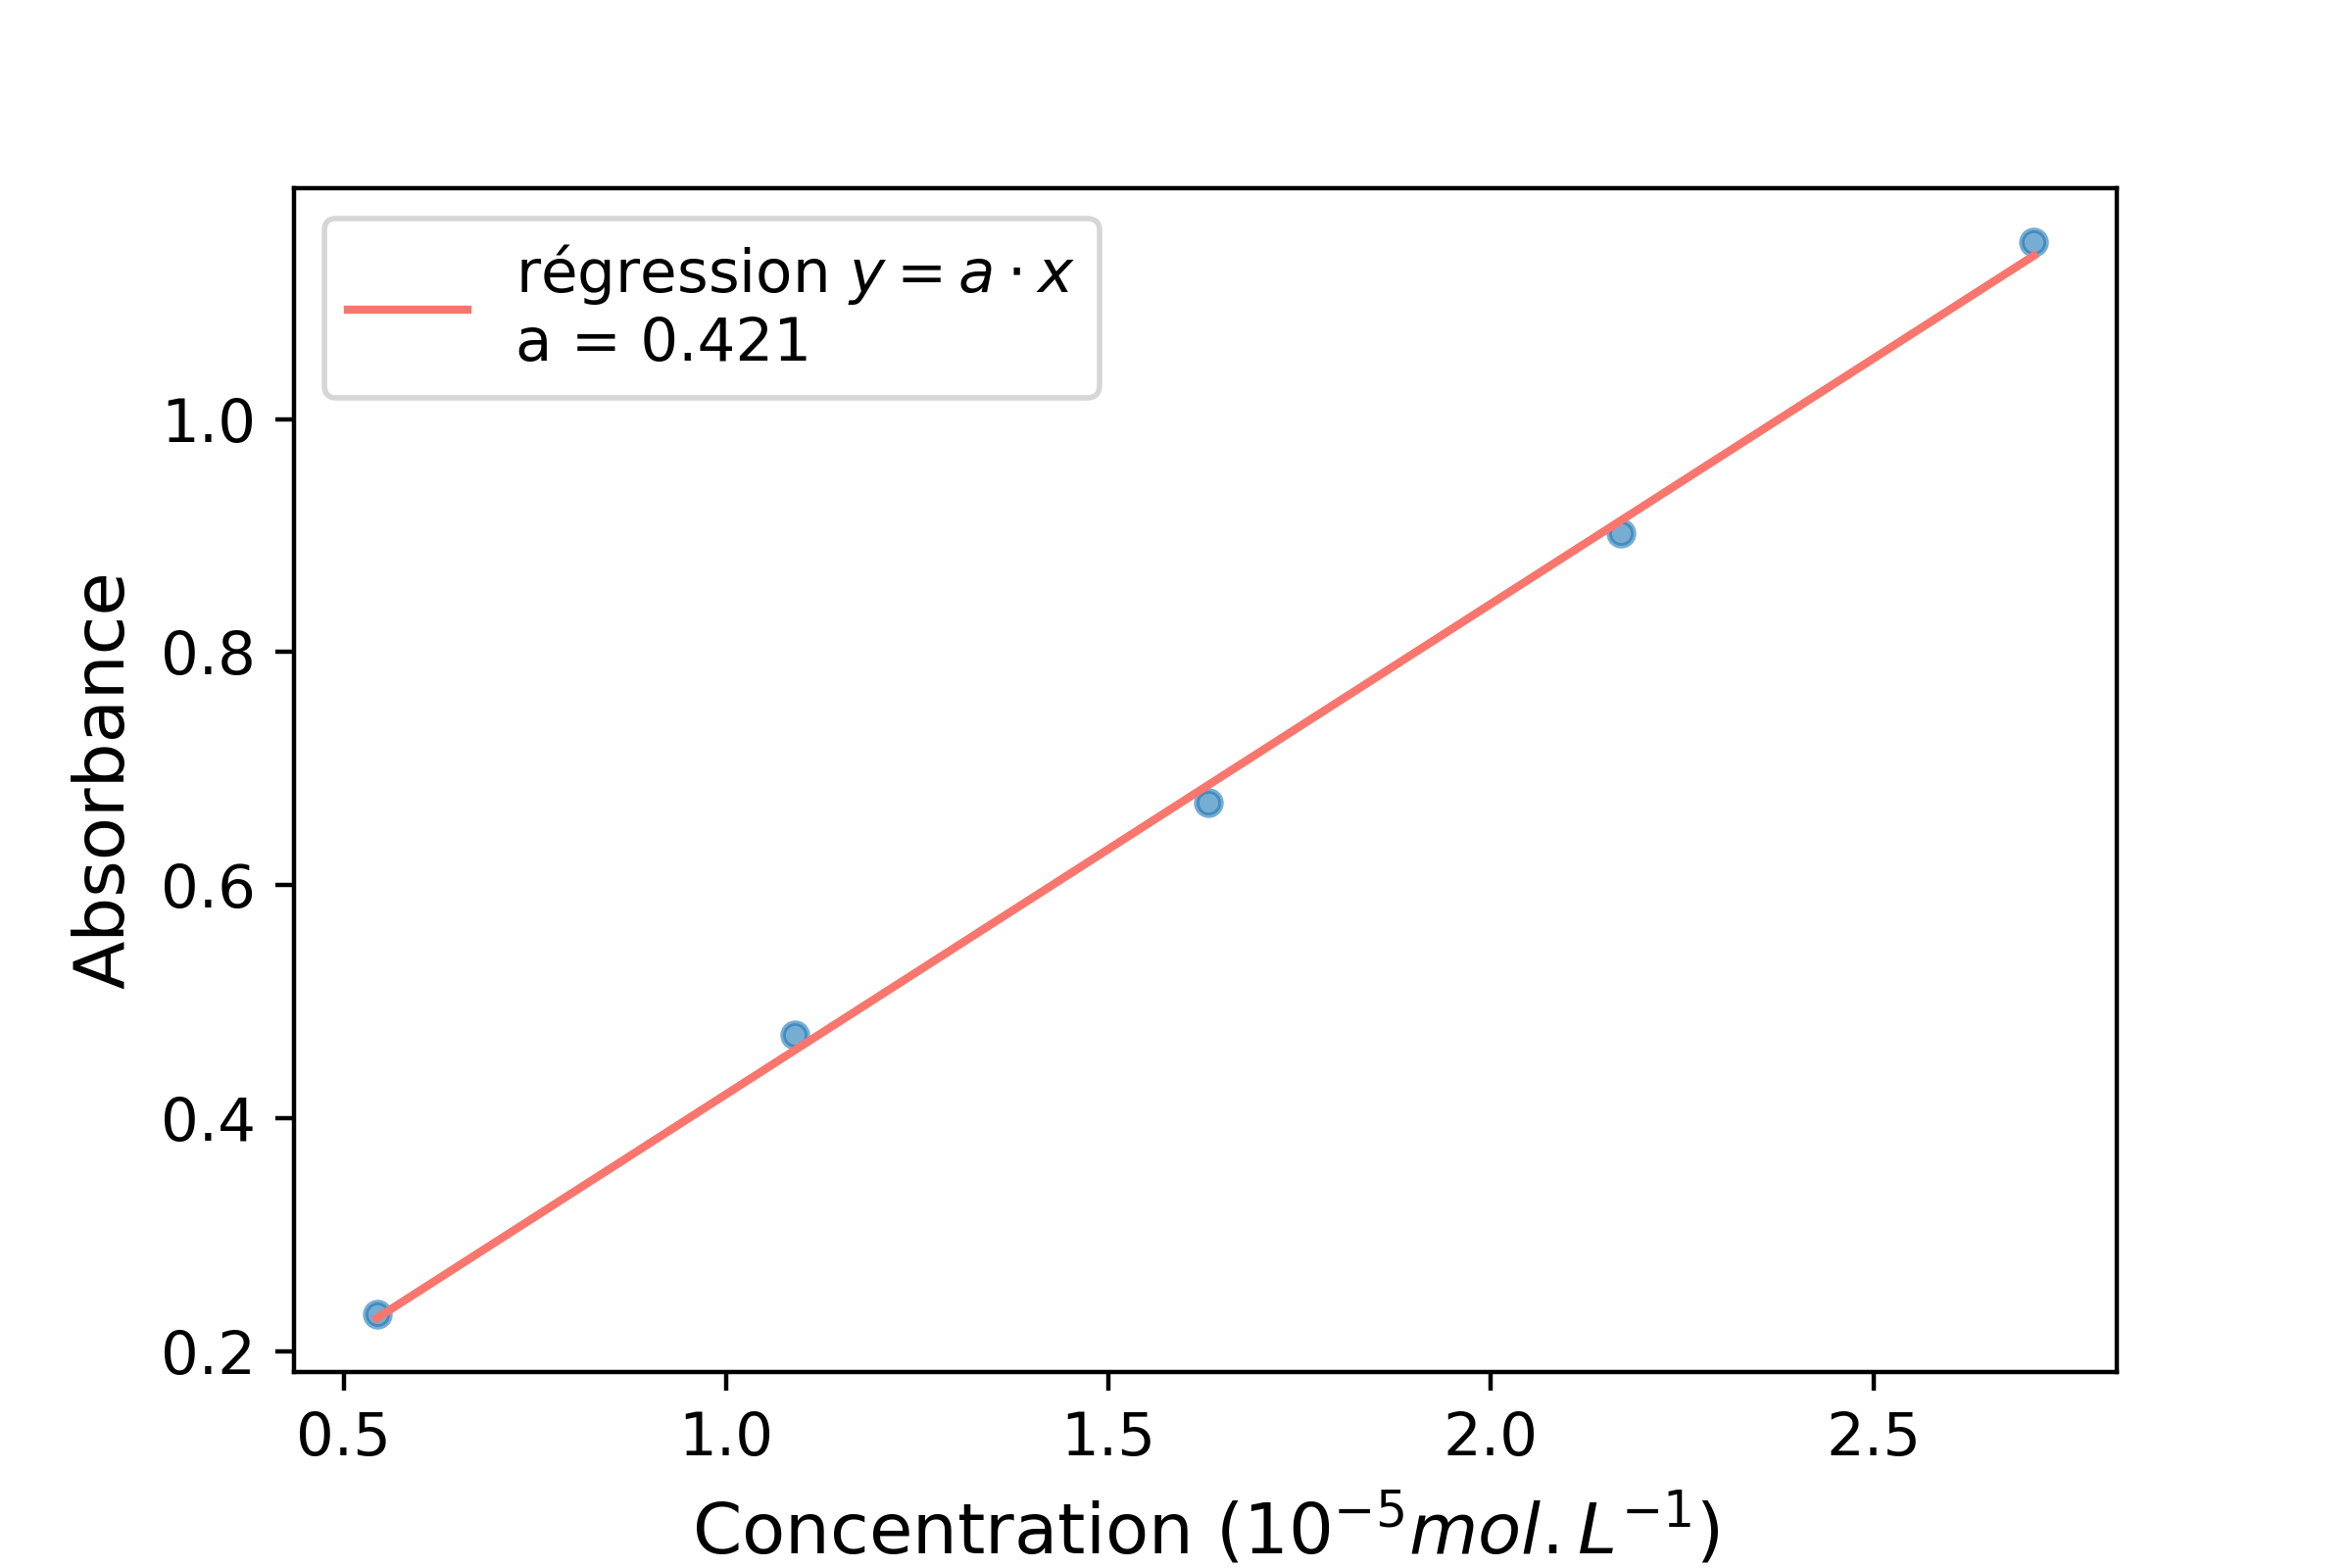
\includegraphics[width = 12cm]{images/regression_Absorbance.png}
\end{center}

A partir du coefficient directeur on peut en déduire le coefficient d'absorption molaire, sachant que la longueur de la cuve est de 1 cm.
%Or l'ajustement donne comme valeur de coefficient directeur $a = (0,421 \pm 0,009) \unit{L.mol^{-1}}$ (incertitude donnée par Régressi). En divisant par la longueur de la cuve ($(1 \pm 0,1) \unit{cm}$), on obtient : $\epsilon = (0,421 \pm 0,043) \unit{L.mol^{-1}.cm^{-1}}$.
\par \textbf{Calcul d'incertitude}
\begin{equation*}
    \frac{\Delta \epsilon}{\epsilon} = \sqrt{\left(\frac{\Delta a}{a}\right)^{2} + \left(\frac{\Delta l}{l}\right)^{2} }
\end{equation*}
\begin{equation*}
    \Delta \epsilon = 0,421 \cdot \sqrt{\left(\frac{0,009}{0,421}\right)^{2} + \left(\frac{0,1}{1}\right)^{2} } = 0,043
\end{equation*}


\end{solution}
\end{framed}

\paragraph{Protocole}

~

Dans un erlenmeyer de 50 mL contenant un barreau aimanté, introduire environ précisément 0,5 g de poudre de curcuma. Ajouter 20 mL d’éthanol et agiter pendant 10 min. Dans une fiole jaugée de 50 mL, filtrer la solution hétérogène. Rincer le solide avec de petites portions d'éthanol. Compléter au trait de jauge et homogénéiser. On obtient alors la \textbf{solution A'}.

\par Dans une fiole jaugée de 100 mL contenant 1 mL d’acide acétique glacial, diluer la solution A’ d’un  facteur 100 (\textbf{solution B'})

\begin{framed}
    \question Déterminer le pourcentage massique de curcumin contenu dans la poudre commerciale de curcuma, avec son incertitude. Comparer à l'indication sur l'étiquette.
    \begin{solution}[8cm]
        On mesure l'absorbance de la solution B', cette mesure donne une valeur de A = 0,435 nm.
        \begin{equation*}
            C_m(A') = \frac{A}{a} \cdot M(\ce{C21H20O6}) \cdot 100
                    = \frac{0,435}{0,421} \cdot 368,38 \cdot 100
                    = 0,381 \unit{g.L^{-1}}
        \end{equation*}
    En notant $m_0$ la masse de curcuma pesée, autour de 0,5 g : 
    \begin{equation*}
          \%_{massique} = \frac{m(A')}{m_0} \cdot 100 = \frac{Cm(A')\cdot V_{A'}}{m_0}
          \cdot 100 = \frac{0,381 \cdot 50.10^{-3}}{0,5} \cdot 100
          = 3,81 \%
    \end{equation*}
  La source d'erreur principale à considérer ici est celle sur la détermination de $C_m(B')$, soit sur la pente de la droite d'étalonnage. Ainsi :
  \begin{equation*}
      \Delta m(A') = \frac{\Delta a}{a} \cdot m(A')
      = 4,07.10^{-4} g
  \end{equation*}
  Donc $\%_{massique} = (3,81 \pm 0,08) \%$
    \end{solution}
\end{framed}






    
\end{questions}

\newpage

\section{Analyse d'une boisson anti-fatigue désaltérante}

La boisson étudiée est constituée de deux composés naturels : l'acide citrique, contenu dans les agrumes, responsable de l'effet désaltérant et la vitamine C, appelée aussi acide ascorbique, contenue dans de nombreux fruits. Cette vitamine intervient dans le cycle de formation de l'adénosine triphosphate, une molécule qui fournit l'énergie lors des processus biochimiques de métabolisme, de transport ou encore de division cellulaire et qui donc aura un effet anti-fatigue. Cette boisson est supposée constituée à 0,15\% massique d'acide citrique et à 0,35\% massique d'acide ascorbique (figure \ref{fig:acides}).

\begin{center}
    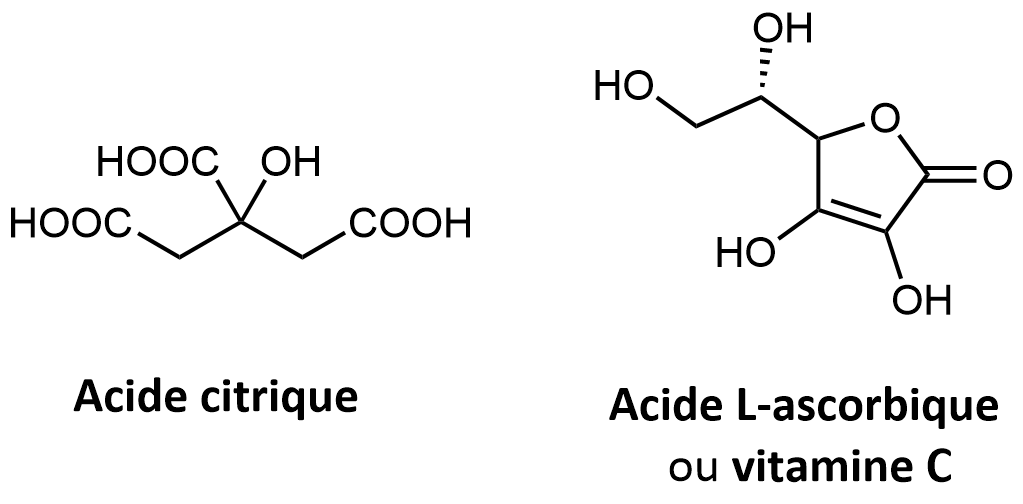
\includegraphics[scale = 0.3]{images/acides.png}
    \captionof{figure}{Composés contenus dans la boisson anti-fatigue}
    \label{fig:acides}
\end{center}

\begin{questions}
    

\begin{framed}
\question Quel est le proton le plus acide de l'acide ascorbique ? Justifier.
\begin{solution}[3cm]
Il s'agit du proton acide dont la base conjuguée est stabilisée par mésomérie.
\begin{center}
    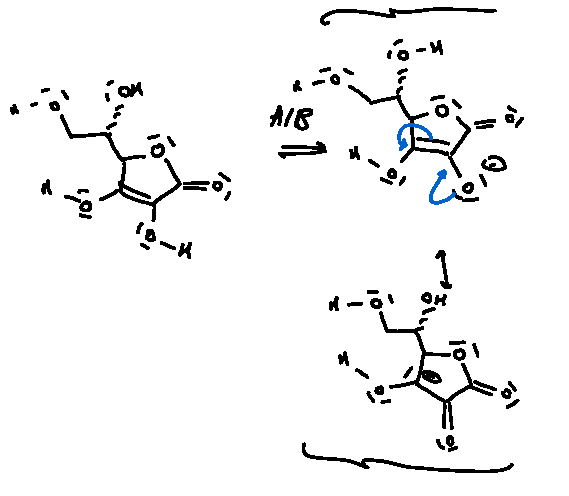
\includegraphics[width = 10cm]{images/proton_vitamine_C.pdf}
\par En regardant la valeur des pKa en annexe, on voit que seule cette acidité sera dosée dans l'eau. 
\end{center}
\end{solution}
\end{framed}


\end{questions}

\par Proposer un protocole pour déterminer la concentration de chacun des deux composés dans la boisson étudiée. On dispose d'une solution d'hydroxyde de sodium à 0,05 \unit{\mol\per\liter}, d'une solution de diiode à 0,05 \unit{\mol\per\liter}, d'une solution d'acide sulfurique à 0,1 \unit{\mol\per\liter} ainsi que de divers indicateurs colorés, et de données sur les composés étudiés (voir l'annexe). 
%Le logiciel \emph{dozzzaqueux} peut également être utilisé.



\textit{Après validation par un examinateur du protocole, mettre en œuvre la manipulation.}

\begin{framed}
    \begin{solution}[7cm]
    Les deux composés ont des propriétés acides. On dose donc dans un premier temps toutes les acidités, puis on dose spécifiquement la vitamine C. On détermine alors par soustraction la quantité d'acide citrique.
    \end{solution}
\end{framed}




\begin{framed}


\begin{solution}[15cm]



\paragraph*{Dosage de toutes les acidités}
~
\par Introduire dans la burette la solution d’hydroxyde de sodium. Dans un bécher de 200 mL, introduire une prise d’essai de 10 mL de la solution à analyser. 
On peut suivre le dosage par pH-métrie ou par colorimétrie avec la phénolphtaléine. 
Le volume équivalent est attendu vers 8,7 mL.
Attention, si l'élève choisit un suivi pH-métrique, le volume équivalent ne peut être déterminé par la méthode des tangentes car le saut n'est pas symétrique.

\begin{center}
    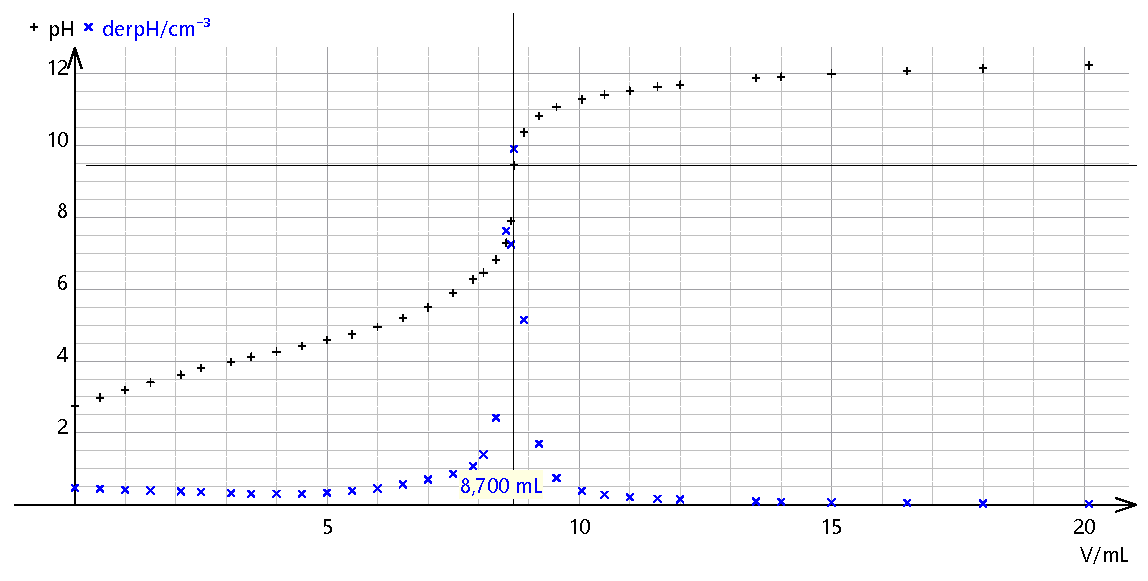
\includegraphics[width = 16cm]{images/graphe_phmetrie.pdf}
    \captionof{figure}{Courbe expérimentale du titrage pH-métrique}
\end{center}

\paragraph*{Dosage de l'acide ascorbique}

~

\par Introduire dans la burette la solution d'acide ascorbique et citrique.
Dans un erlenmeyer de 150 mL, introduire une prise d’essai de 5 mL de solution de diiode. Ajouter environ 20 mL d'acide sulfurique à 0,1 \unit{\mol\per\liter} afin d'être dans le domaine de stabilité du diiode. Réaliser le dosage : lorsque la solution devient jaune pâle, ajouter une pointe de spatule de thiodène. Le volume équivalent est attendu vers 12,5 mL.

\paragraph{Détermination des concentrations}

~

\par $C_1$ = concentration en acide citrique
\par $C_2$ = concentration en acide ascorbique


\begin{equation*}
    C_2 = \frac{C_{\ce{I2}} \cdot V_0'}{V_{eq}^{2}} = \frac{0,05 \cdot 5}{12,5} = 0,02 \ \unit{mol.L^{-1}}
\end{equation*}

On pose $C{t}$ la concentration de la solution de soude.

\begin{equation*}
    C_1 = \frac{C_{t} \cdot V_{eq}^{1} - C_2 \cdot V_0}{3 V_0} = \frac{0,05 \cdot 8,7 - 0,02 \cdot 10}{3 \cdot 10} = 7,8.10^{-3} \ \unit{mol.L^{-1}}
\end{equation*}

\end{solution}
\end{framed}

\begin{solution}
\paragraph*{Calculs}
\begin{flushleft}
    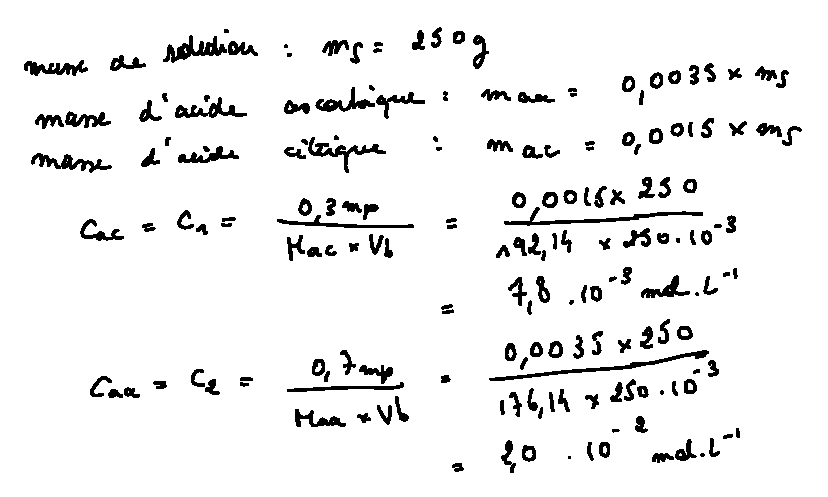
\includegraphics[scale = 0.9]{images/calcul_concentrations_initiales.pdf}
    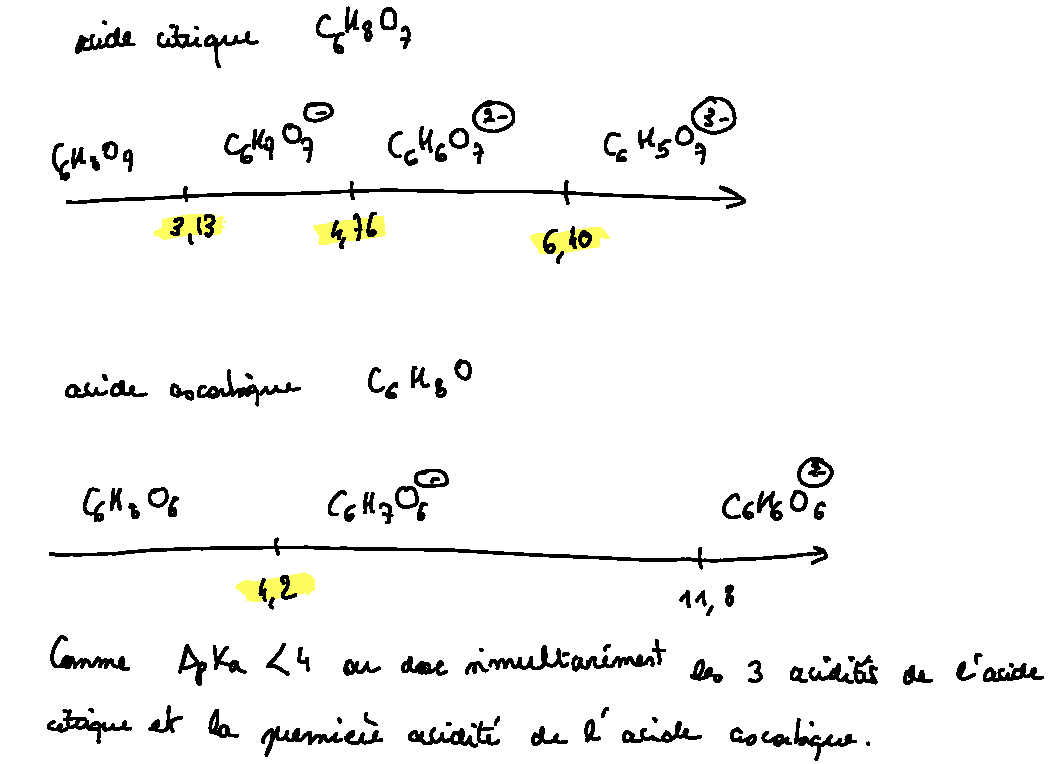
\includegraphics[scale = 0.8]{images/calculs-1.pdf}
    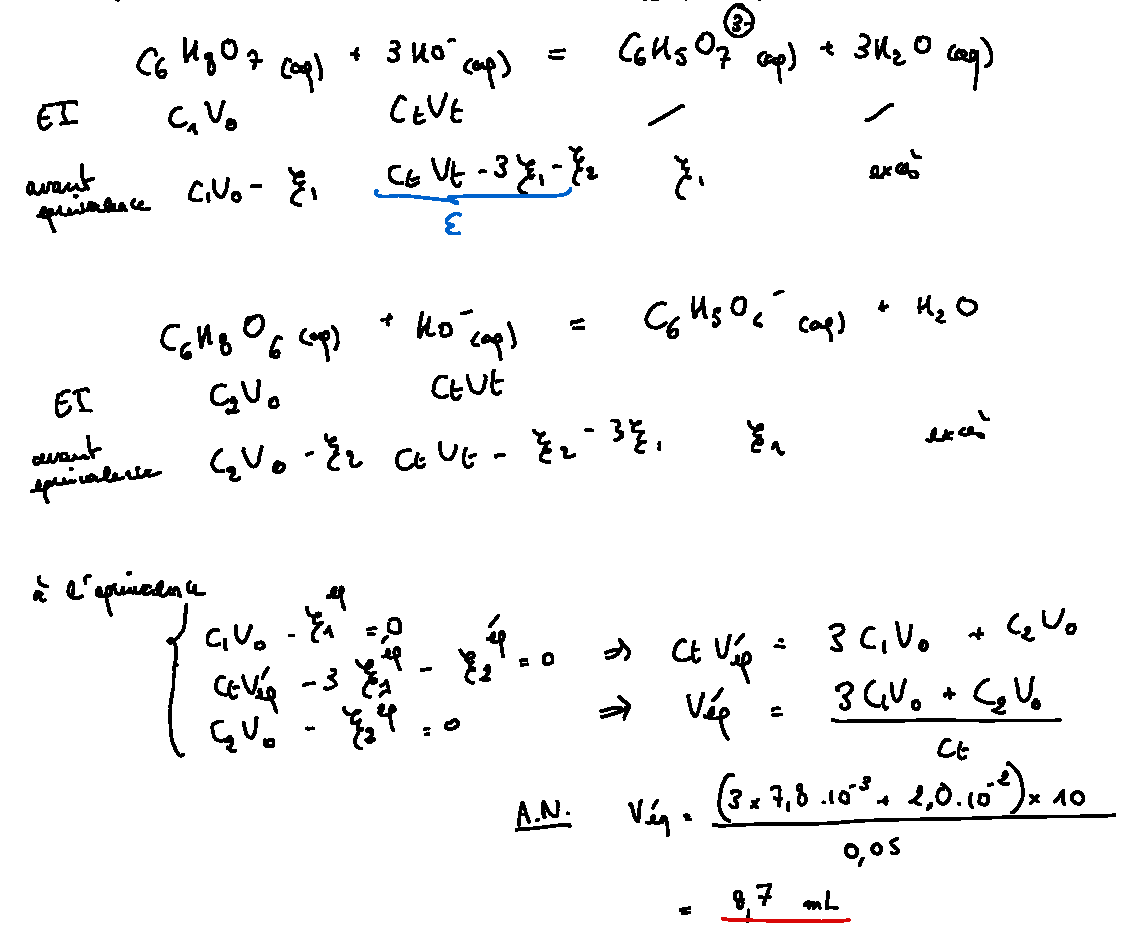
\includegraphics[scale = 0.8]{images/calculs-2.pdf}
    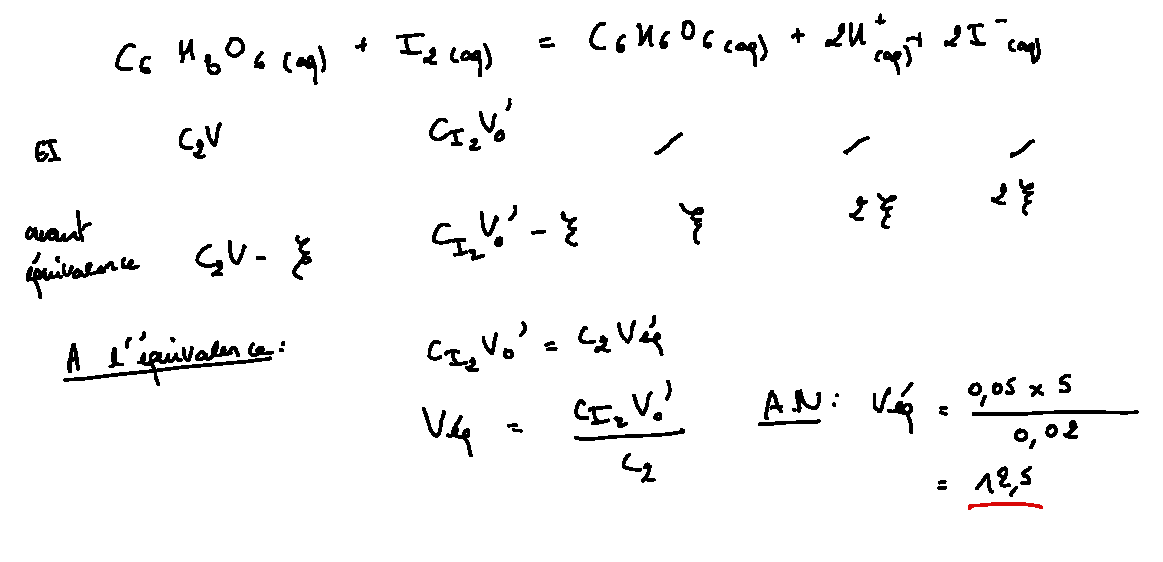
\includegraphics[scale = 0.8]{images/calculs-3.pdf}
\end{flushleft}
%calculer la concentration attendue en chacun + le ph à l'équivalence

\end{solution}








\newpage
\section*{Annexe}\label{sec:annexe}

\subsection*{Données}

\paragraph*{Indice de réfraction tabulé de l'acétate de benzyle} : 1,502 à 25 °C.
% à retirer éventuellement pour les laisser comparer à l'acétate de benzyle commercial.



\paragraph*{Zones de virage de quelques indicateurs colorés acido-basiques}:
\begin{itemize}
    \item Bleu de bromothymol : 6-7,6
    \item Rouge de méthyle : 4.2-6.2
    \item Phenolphtaléine : 8-9.8
\end{itemize}

~

\par Le thiodène est un indicateur coloré redox, incolore, qui prend une couleur bleu foncé en présence de diiode.

\paragraph*{pK$_a$ de quelques acides étudiés}:
\begin{itemize}
    \item Acide citrique : \quad 3,13 \quad ;  \quad 4,76 \quad ; \quad 6,40
    \item Acide ascorbique : \quad 4,2 \quad ; \quad 11,8
\end{itemize}

\paragraph*{Potentiels standard à 25°C, par rapport à l'électrode standard à hydrogène (ESH)}
\begin{itemize}
    \item $E^{o}_{\ce{I2}/\ce{I-}} = 0,62 V_{/ESH}$
    \item $E^{o}_{AD/AA} = 0,13 V_{/ESH}$
\end{itemize}

~

\par AA : Acide ascorbique (\ce{C6H8O6})
\par AD : acide déshydroascorbique (\ce{C6H6O6})

\paragraph*{Structure de l'APTS}
\begin{center}
    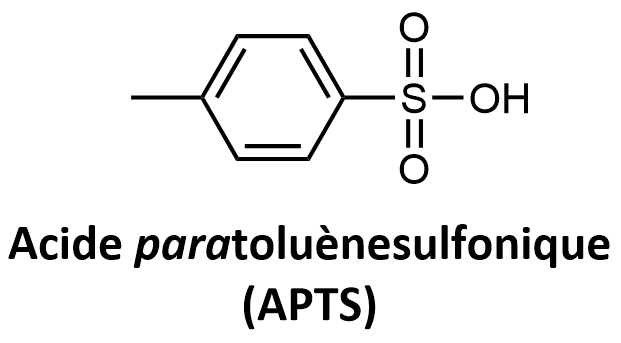
\includegraphics[scale = 0.3]{images/APTS.png}
\end{center}

%rajouter le diagramme E-pH du diiode.
\begin{table}[htbp]
    \centering
    \begin{tabular}{|c|c|c|c|c|}
         \hline
            & C & H & O & S \\
        \hline
        Masse molaire ($~\ch{g\cdot mol^{-1}}$) & 12,01 & 1,01 & 16,00 & 32,06 \\
\hline 
    \end{tabular}
    \caption{Masses molaires de certains éléments}
    \label{tab:MM}
\end{table}

\begin{table}[htbp]
    \centering
    \begin{tabular}{|c|c|c|}
    \hline
         Composé & Densité & $T_{eb}$ (°C) \\
         \hline
         Acide acétique & 1,08 & 117,9 \\
         \hline
         Alcool benzylique & 1,04 & 205,3 \\
         \hline
         Éther diéthylique & 0,71 & 35 \\
         \hline
         Cyclohexane & 0,78 & 80,8 \\
         \hline
         Acétate d'éthyle & 0,90 & 77,1  \\
         \hline        
    \end{tabular}
    \caption{Densités à 25°C et températures d'ébullition de quelques liquides à $P_{atm}$}
    \label{tab:my_label}
\end{table}



\begin{center}
    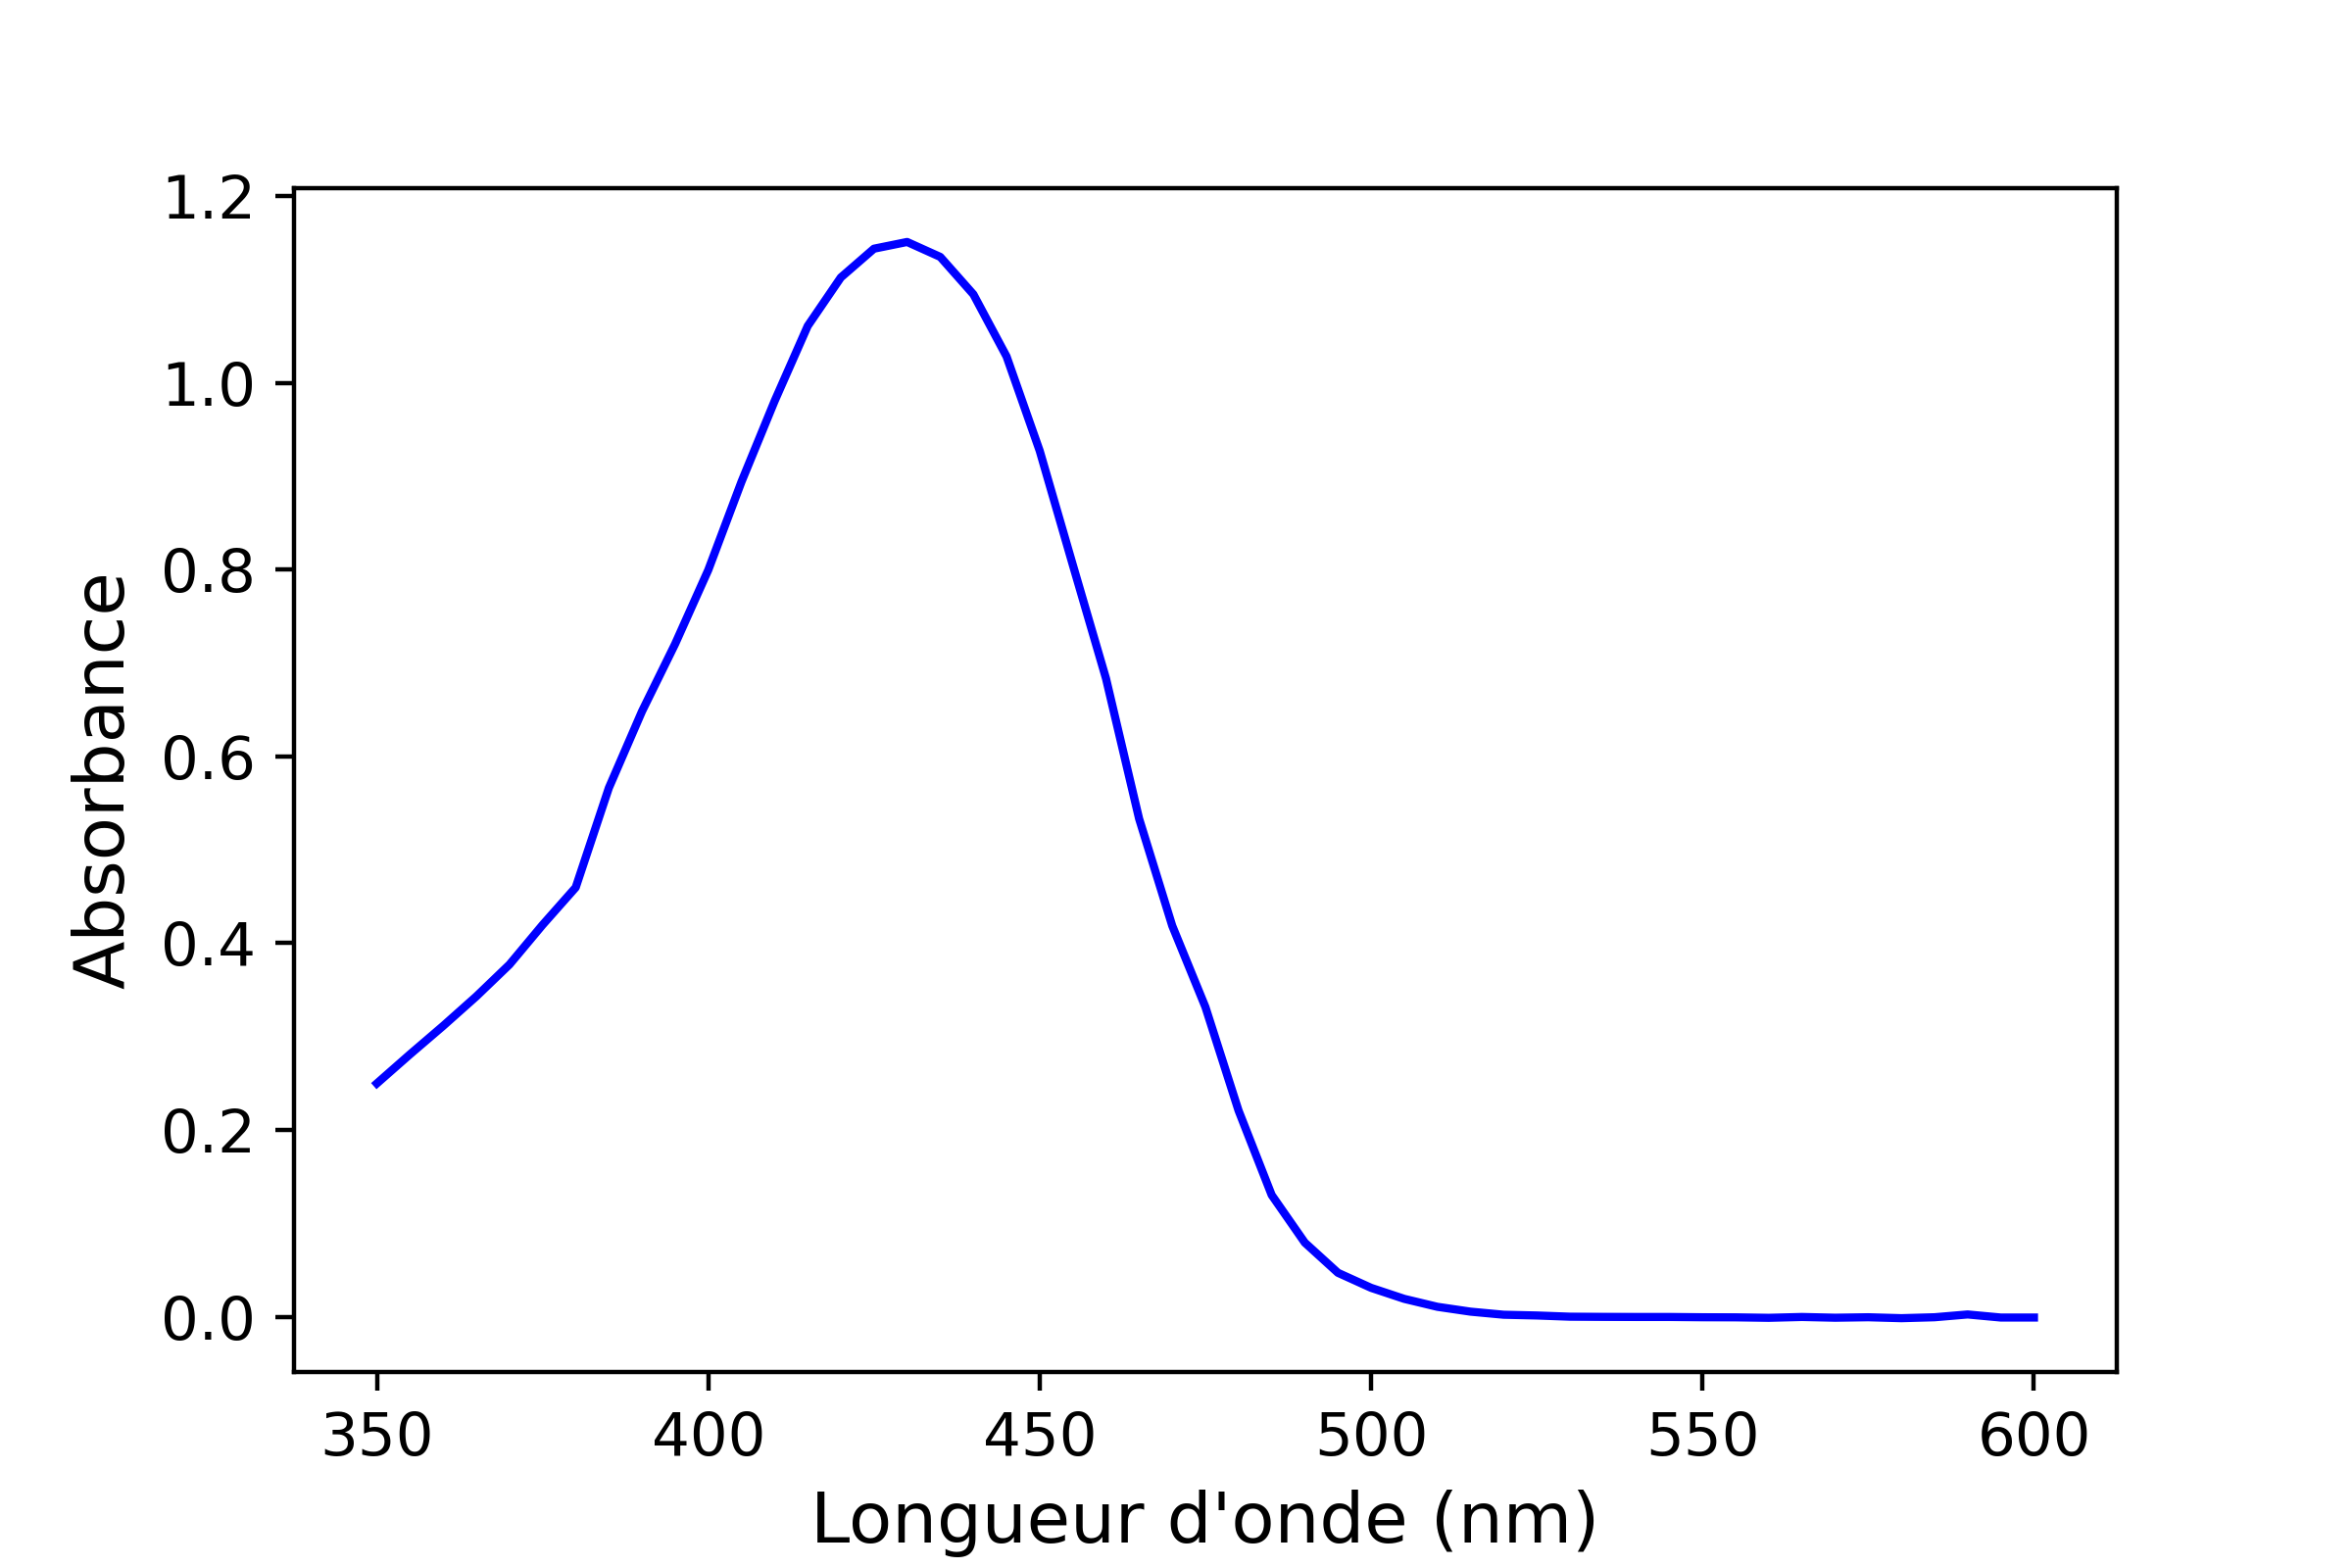
\includegraphics[scale = 0.8]{images/spectre_curcumin.png}
    \captionof{figure}{Spectre d'absorption du curcumin}
    \label{fig:spectre_curcumin}
\end{center}

\begin{center}
    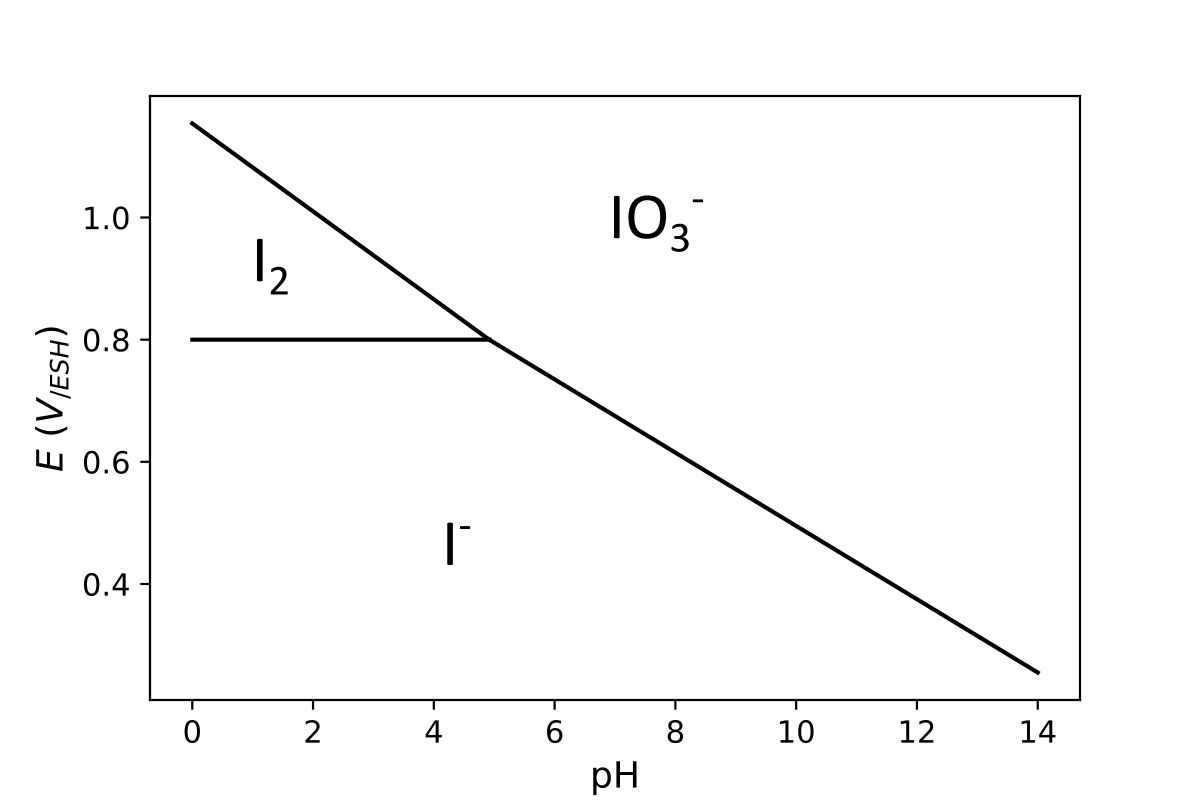
\includegraphics[scale = 0.8]{images/diagramme_EpH_I2.png}
    \captionof{figure}{Diagramme E-pH de l'iode pour une concentration de $10^{-6} \unit{mol.L^{-1}}$}
\end{center}

\newpage
\subsection*{Précautions et risques associés aux produits chimiques utilisés}

\begin{comment}
pictos noms des icônes de danger à remplir à la main dans le tableau : 
- toxic(toxique), 
- skull, 
- flamm, inflammable 
- explo, explosif
- exclam (danger) 
- envi (environnement), 
- corro, corrosif 
- combu, comburant
- cmr,
- bottle (pression)
\end{comment}

\noindent\begin{tabular}{p{6.7cm}p{2cm}p{7cm}rrrrrrrrrr}
\toprule
Produit & Sécurité & Risque (H) Prudence (P) \\
\midrule
Acide éthanoïque glacial \newline (60,05 g/mol) & 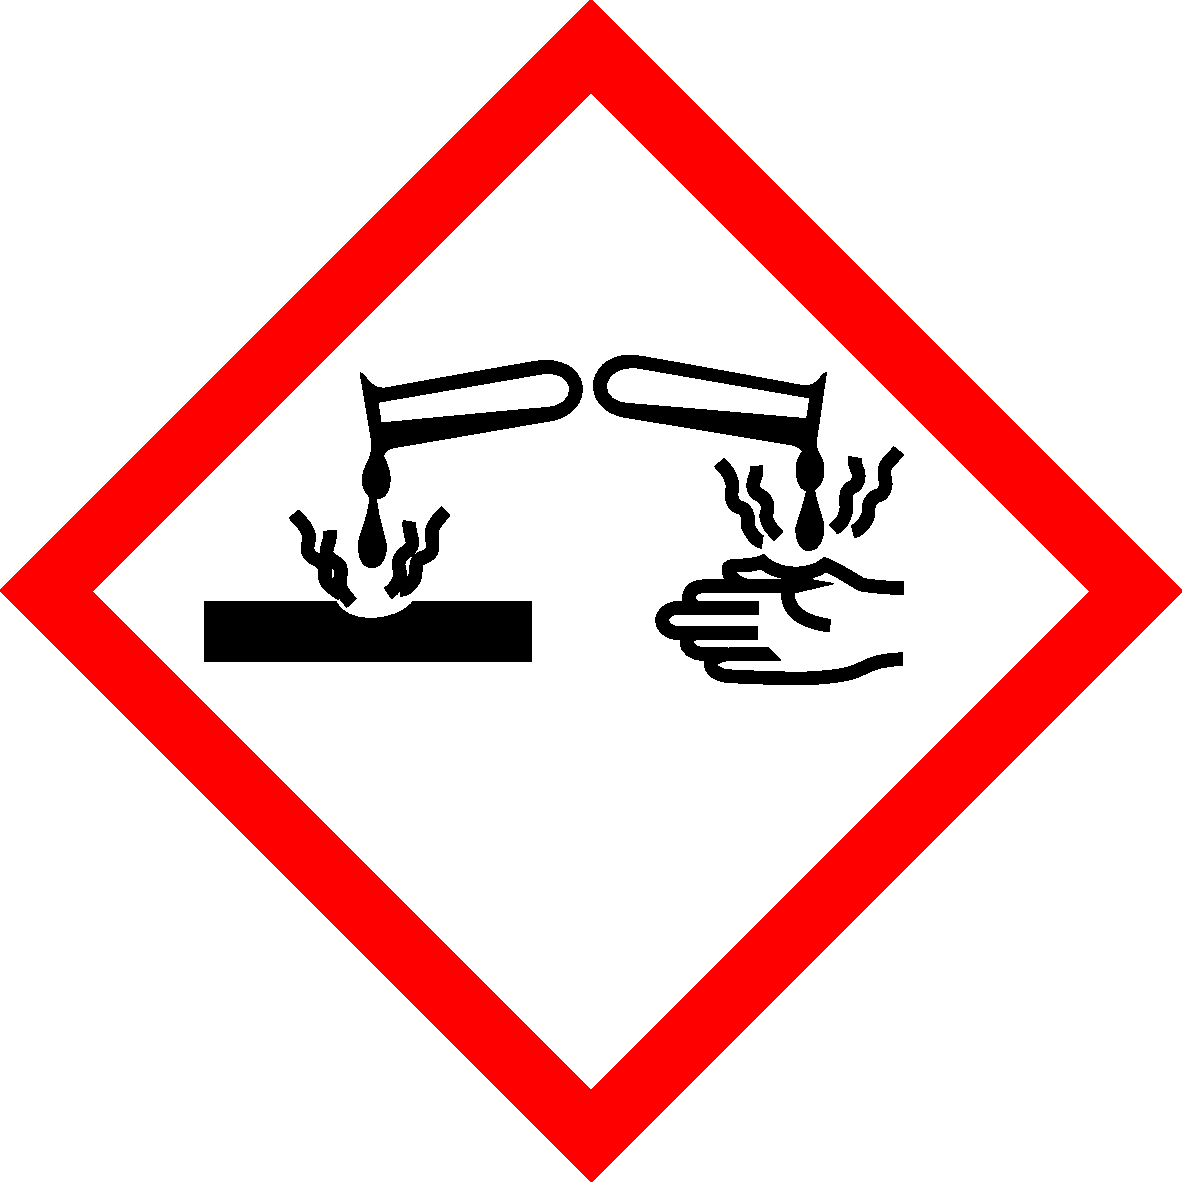
\includegraphics[height=24pt,valign=t]{pictos/corro.pdf}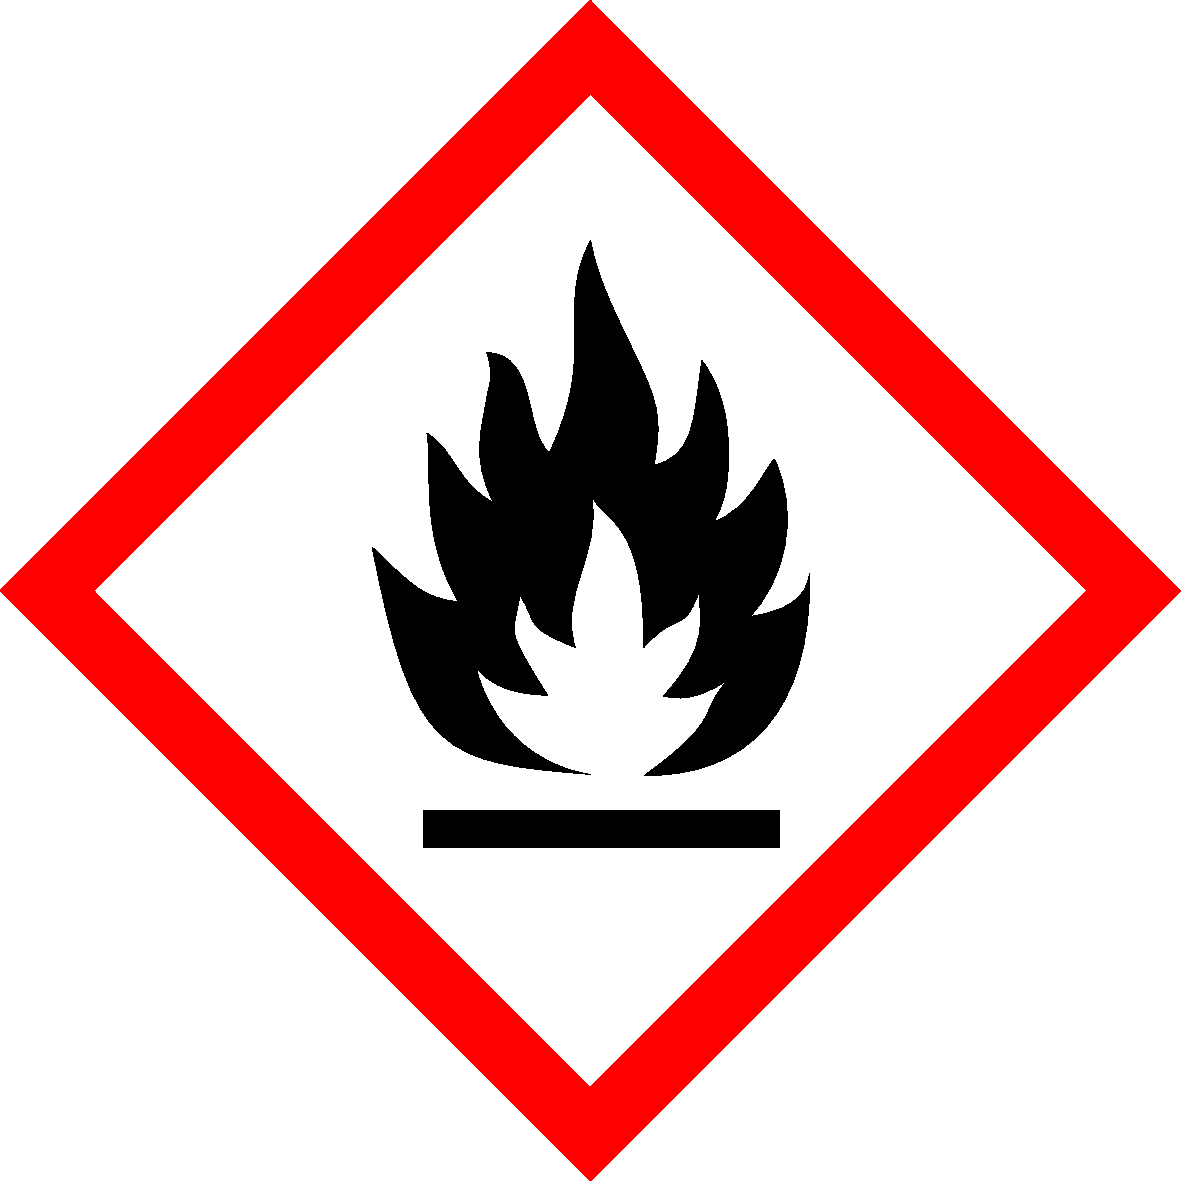
\includegraphics[height=24pt,valign=t]{pictos/flamm.pdf} &  
H226, H314 \newline P210, P233, P240, P280, P303 + P361 + P353, P305 + P351 + P338 \\
\midrule
Alcool benzylique \newline (108,14 g/mol) & 
\includegraphics[height=24pt,valign=t]{pictos/exclam.pdf} &  
H302 + H332, H319 \newline P261, P264, P271, P301 + P312, P304 + P340 + P312, P305 + P351 + P338 \\
\midrule
Acétate de benzyle \newline (150,18 g/mol) & 
\includegraphics[height=24pt,valign=t]{pictos/exclam.pdf}  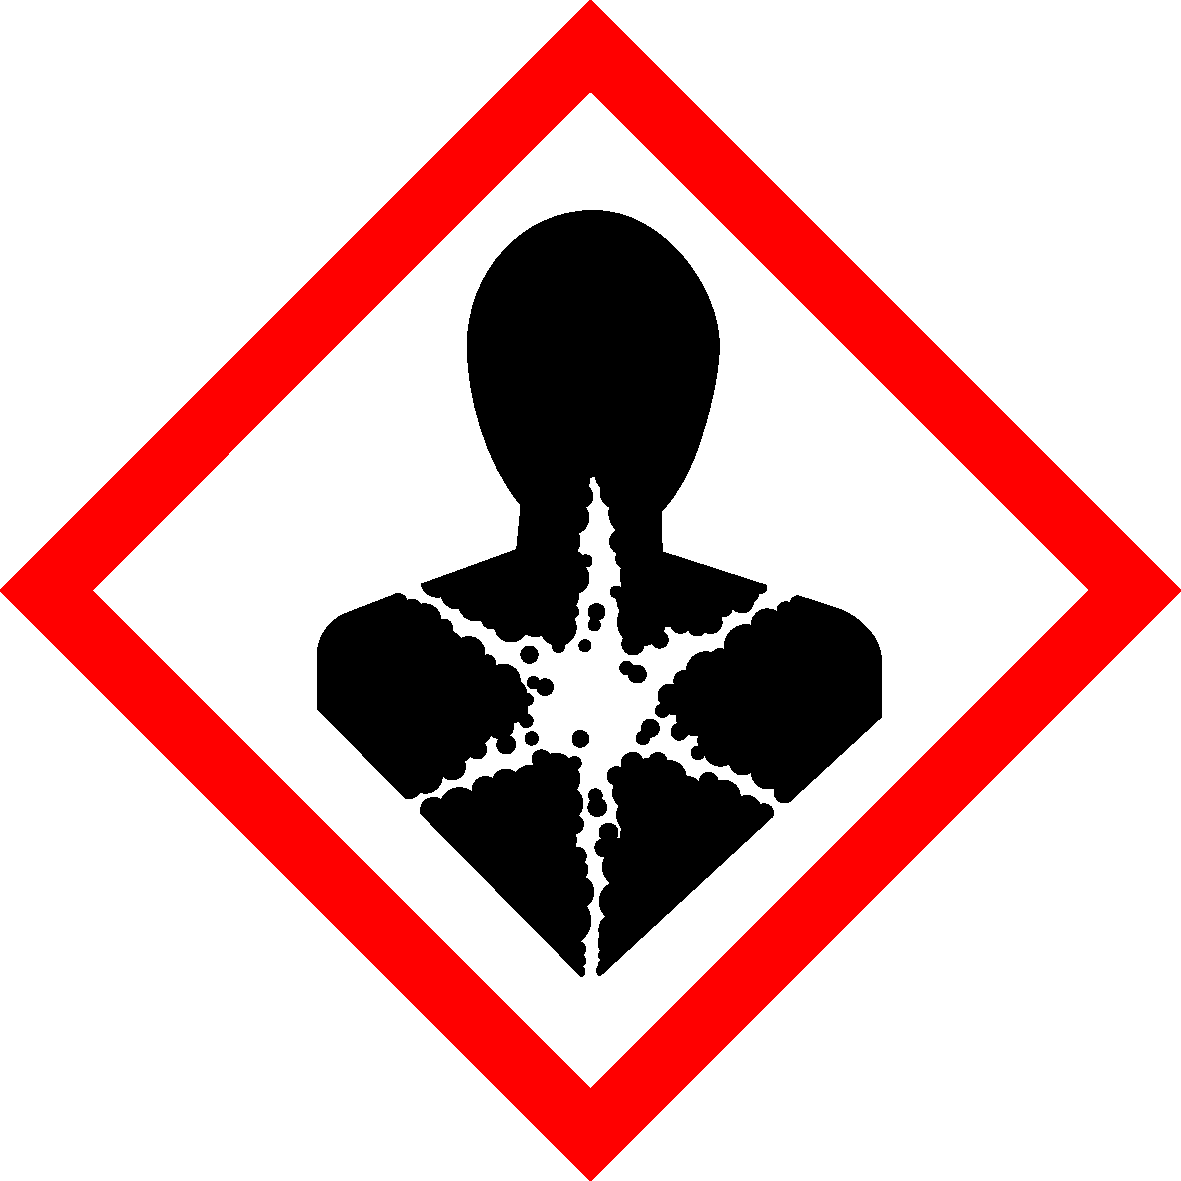
\includegraphics[height=24pt,valign=t]{pictos/cmr.pdf}&  
H319, H335, H315 \newline P261, P280, P302+P352, P305+P351+P338 \\
\midrule
Acide \textit{para}toluènesulfonique (APTS) \newline (190,22 g/mol) & 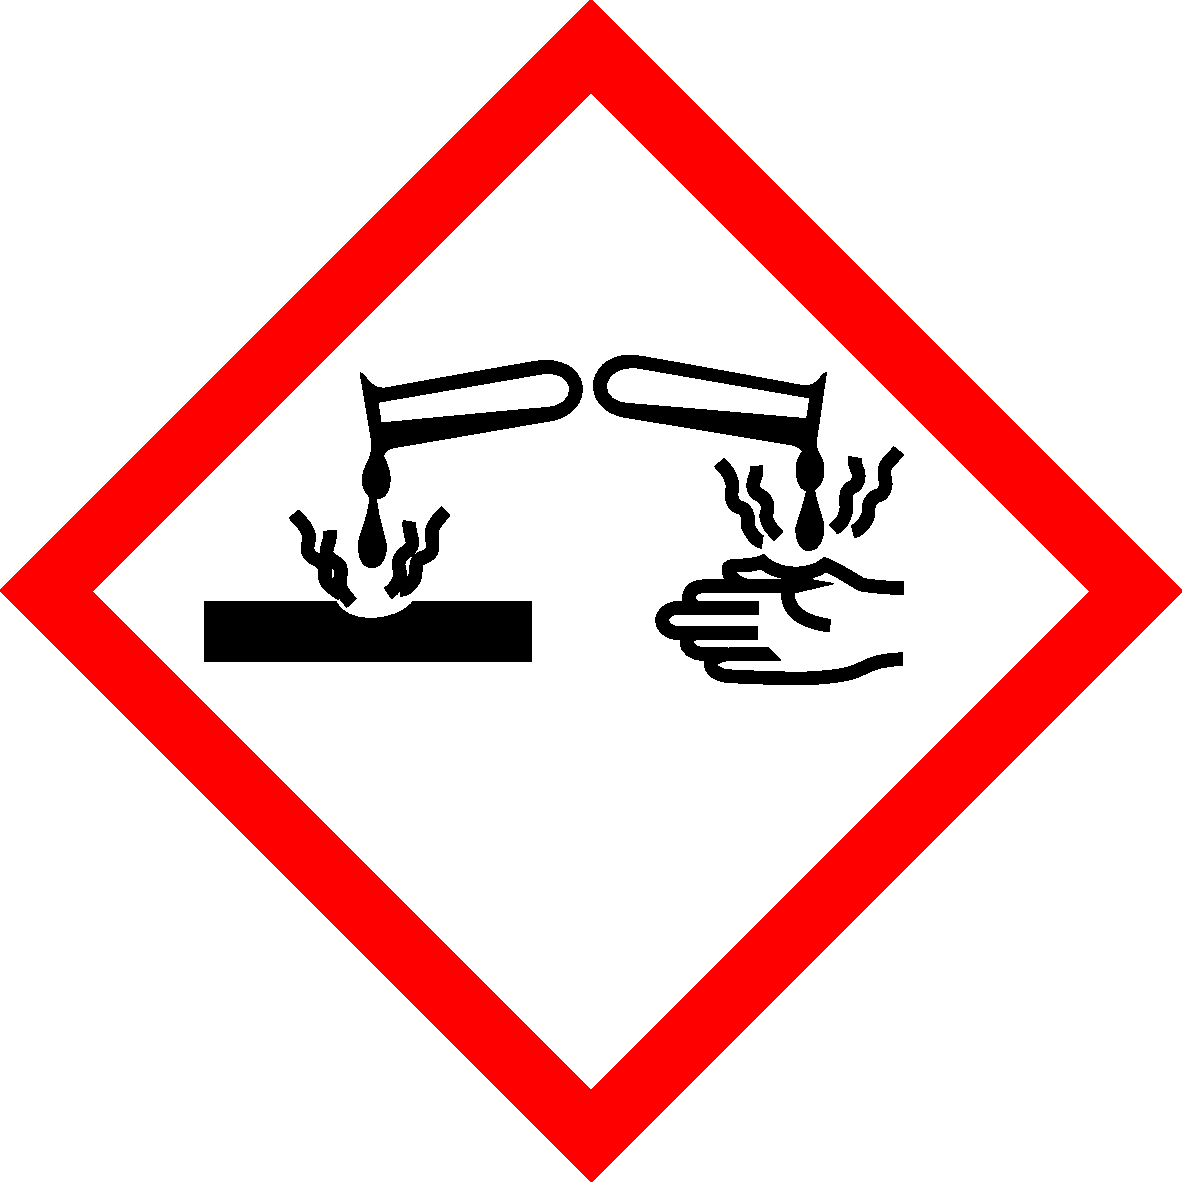
\includegraphics[height=24pt,valign=t]{pictos/corro.pdf}
\includegraphics[height=24pt,valign=t]{pictos/exclam.pdf} &  
H290 , H314 , H335 , H412\newline P234, P260 , P273, P280 , P303 + P361 + P353 , P305 + P351 + P338\\
\midrule
Sulfate de magnésium anhydre \newline (120,37 g/mol) & 
\includegraphics[height=24pt,valign=t]{pictos/exclam.pdf}
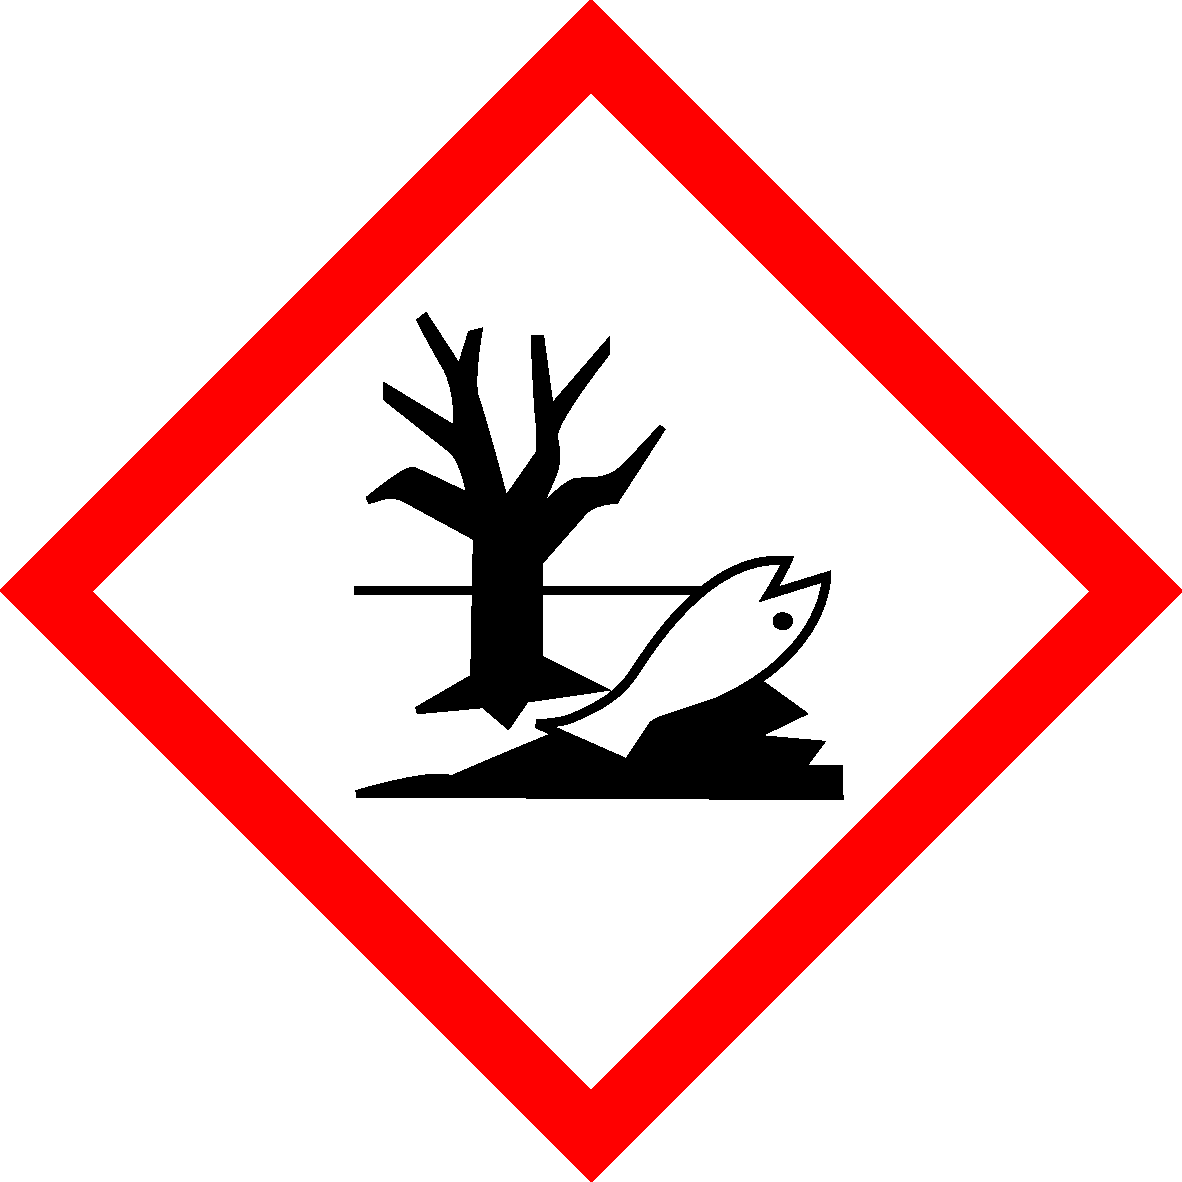
\includegraphics[height=24pt,valign=t]{pictos/envi.pdf} &  
\\
\midrule
Curcumin \newline (368,38 g/mol) & &  
\\
\midrule
Diiode (0,05 \unit{mol.L^{-1}}) \newline (253,81 g/mol) & 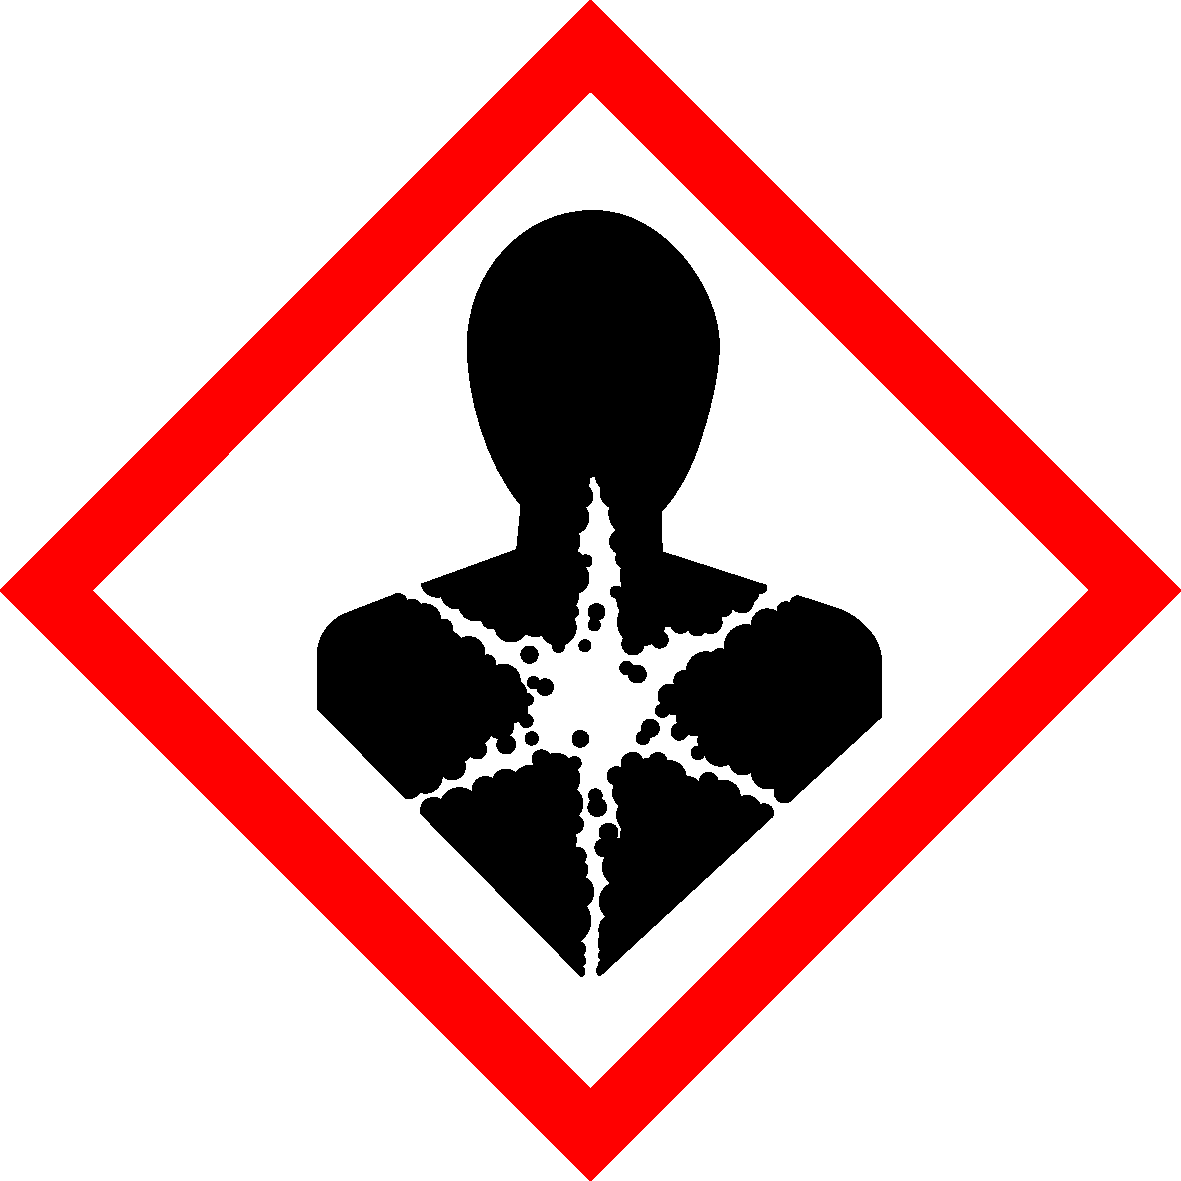
\includegraphics[height=24pt,valign=t]{pictos/cmr.pdf}
\includegraphics[height=24pt,valign=t]{pictos/exclam.pdf} 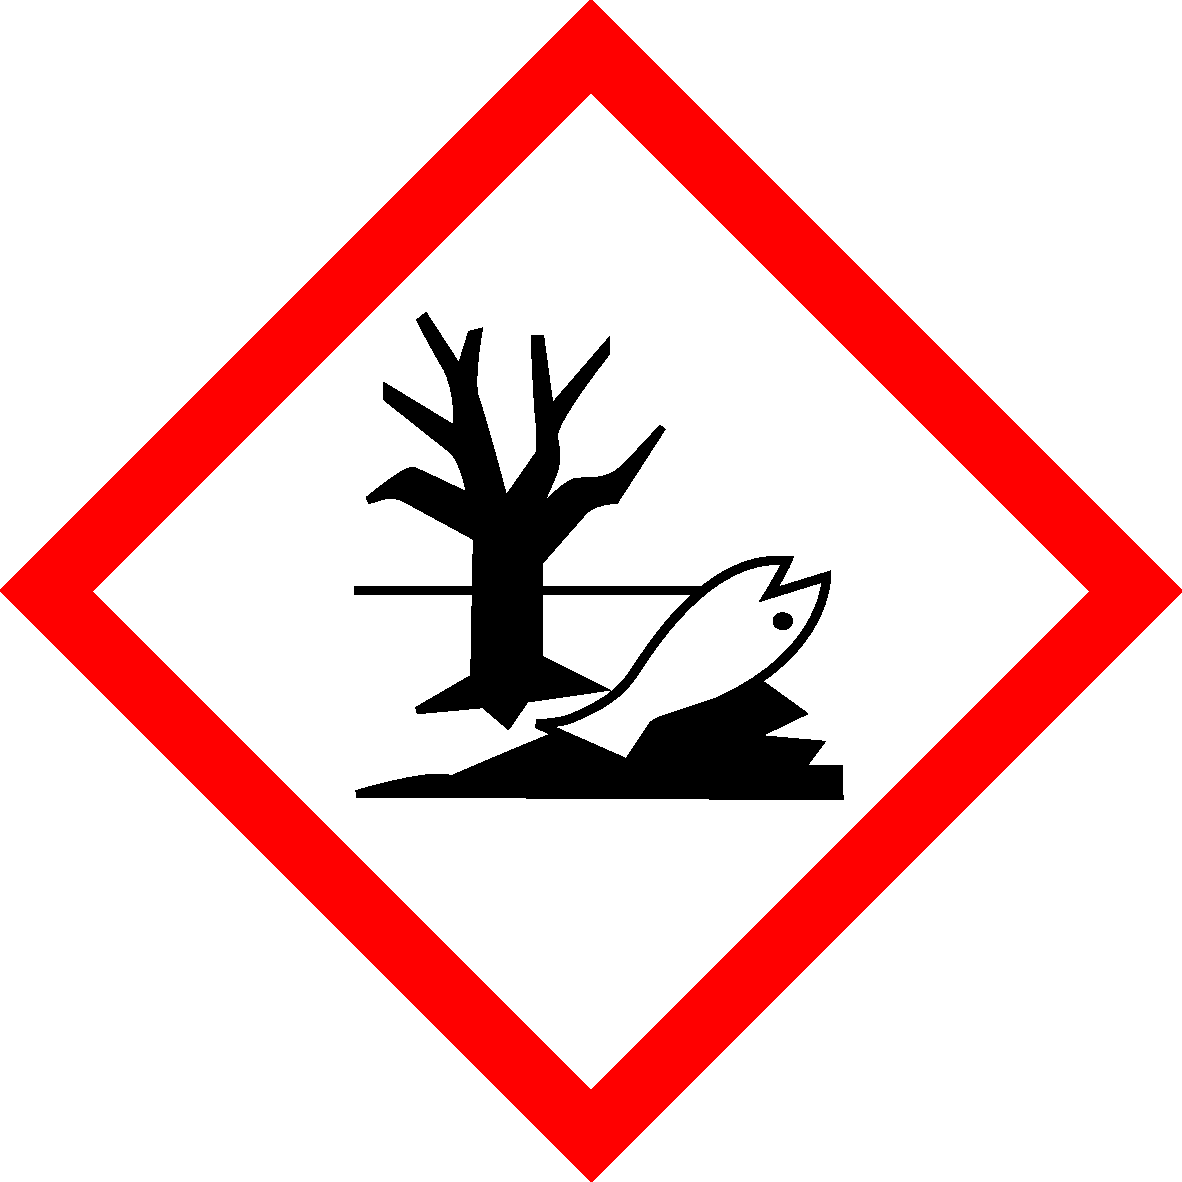
\includegraphics[height=24pt,valign=t]{pictos/envi.pdf} &  
H312, H315, H319, H335, H372, H400\newline P261, P273, P280, P305 + P351 + P338, P314\\
\midrule
Hydroxyde de sodium (0,05 \unit{mol.L^{-1}}) \newline (40,00 g/mol) & 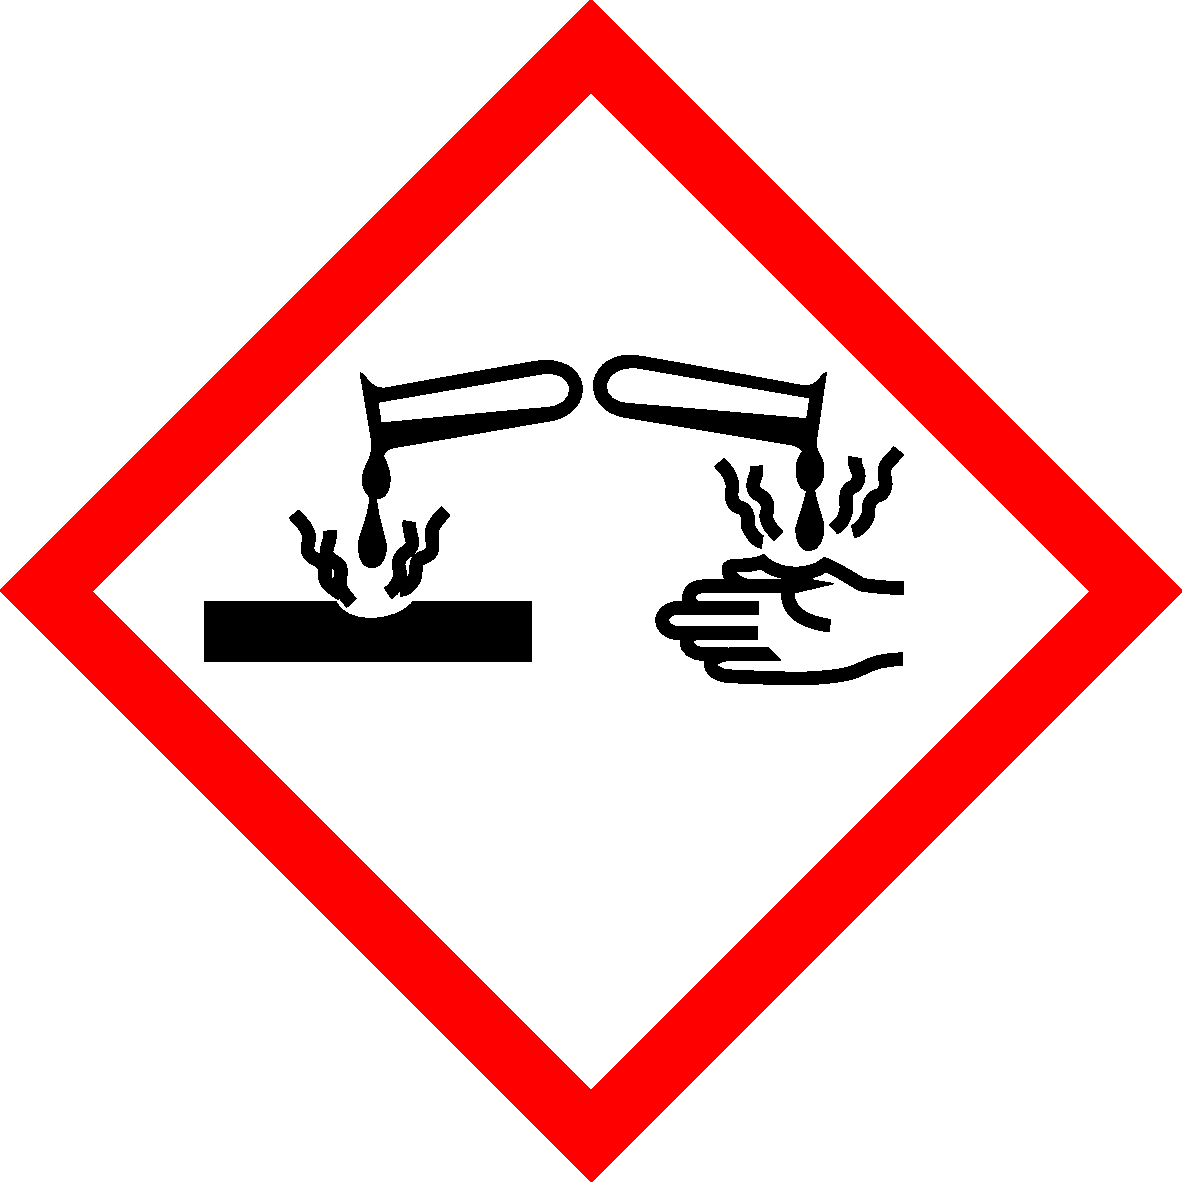
\includegraphics[height=24pt,valign=t]{pictos/corro.pdf} &  
H290, H314 \newline P234, P260, P280, P303 + P361 + P353, P304 + P340 + P310, P305 + P351 + P338 \\
\midrule
Acide citrique \newline (192.12 g/mol) & 
\includegraphics[height=24pt,valign=t]{pictos/exclam.pdf} &  H319, H335 \newline
P261, P264, P271, P280, P304 + P340 + P312, P305 + P351 + P338\\
\midrule
Acide ascorbique \newline (176,12 g/mol) & & \\
\midrule
Acide sulfurique (solution 0,1 \unit{mol.L^{-1}}) \newline (98,08 g/mol) & 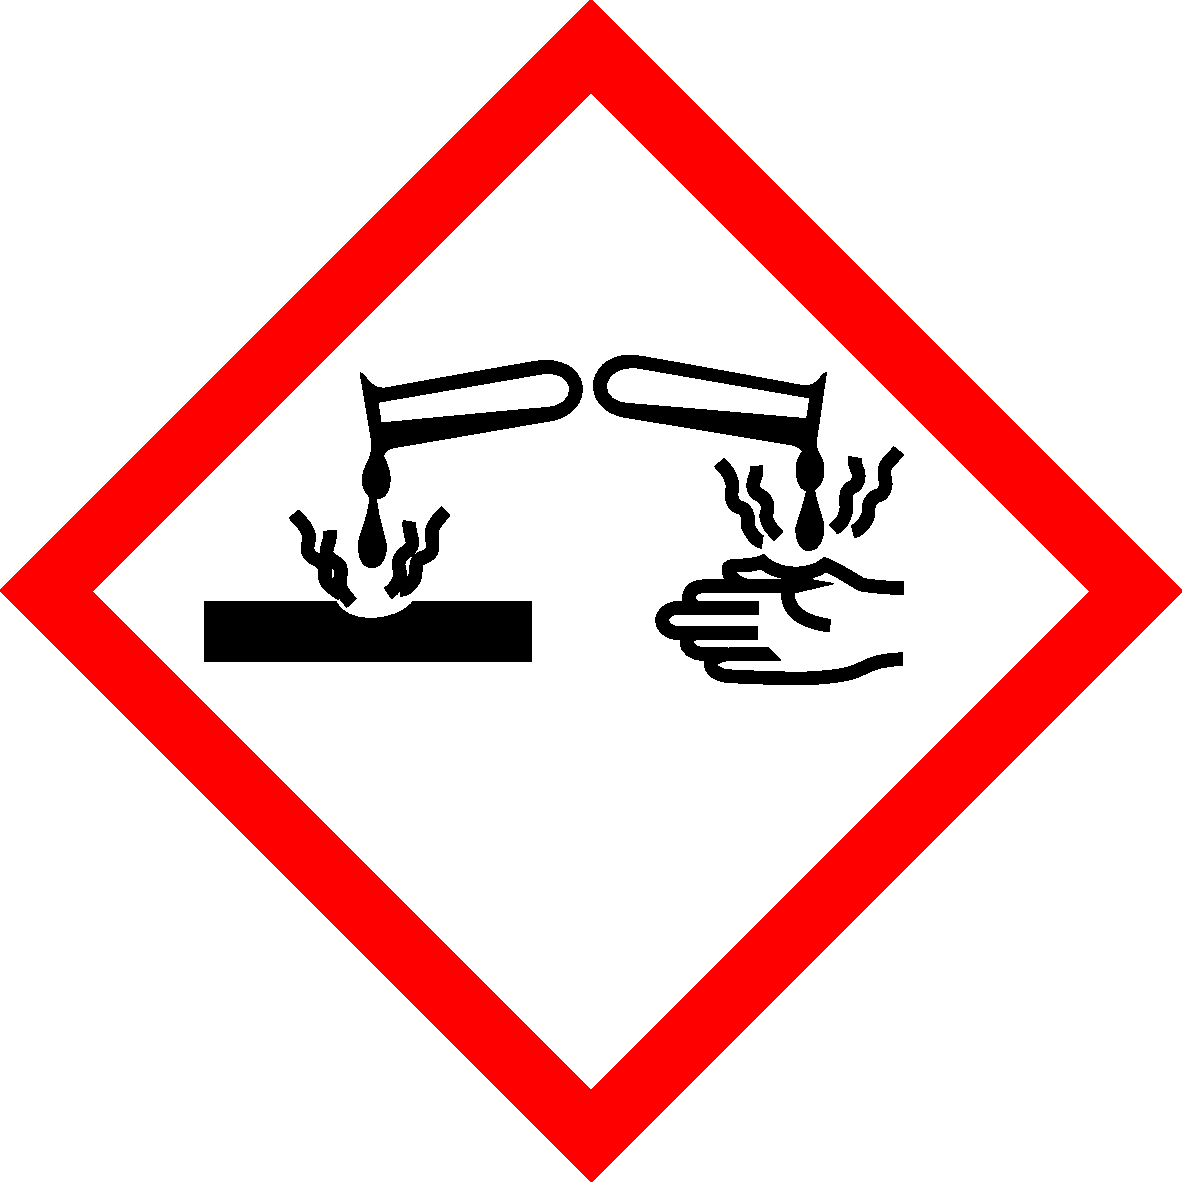
\includegraphics[height=24pt,valign=t]{pictos/corro.pdf} &  H314, H318, H401 \newline
P260, P264, P273, P280, P301 + P330 + P331, P303 + P361 + P353, P304 + P340, P305 + P351 + P338, P310, P363, P405, P501\\
\midrule
Hydrogénocarbonate de sodium (solution saturée) \newline (84,01g/mol) & &  \\
\midrule
Chlorure de sodium (solution saturée) \newline (58,44 g/mol) & &  \\
\midrule
Bleu de bromothymol, solution \newline (624,40 g/mol) & 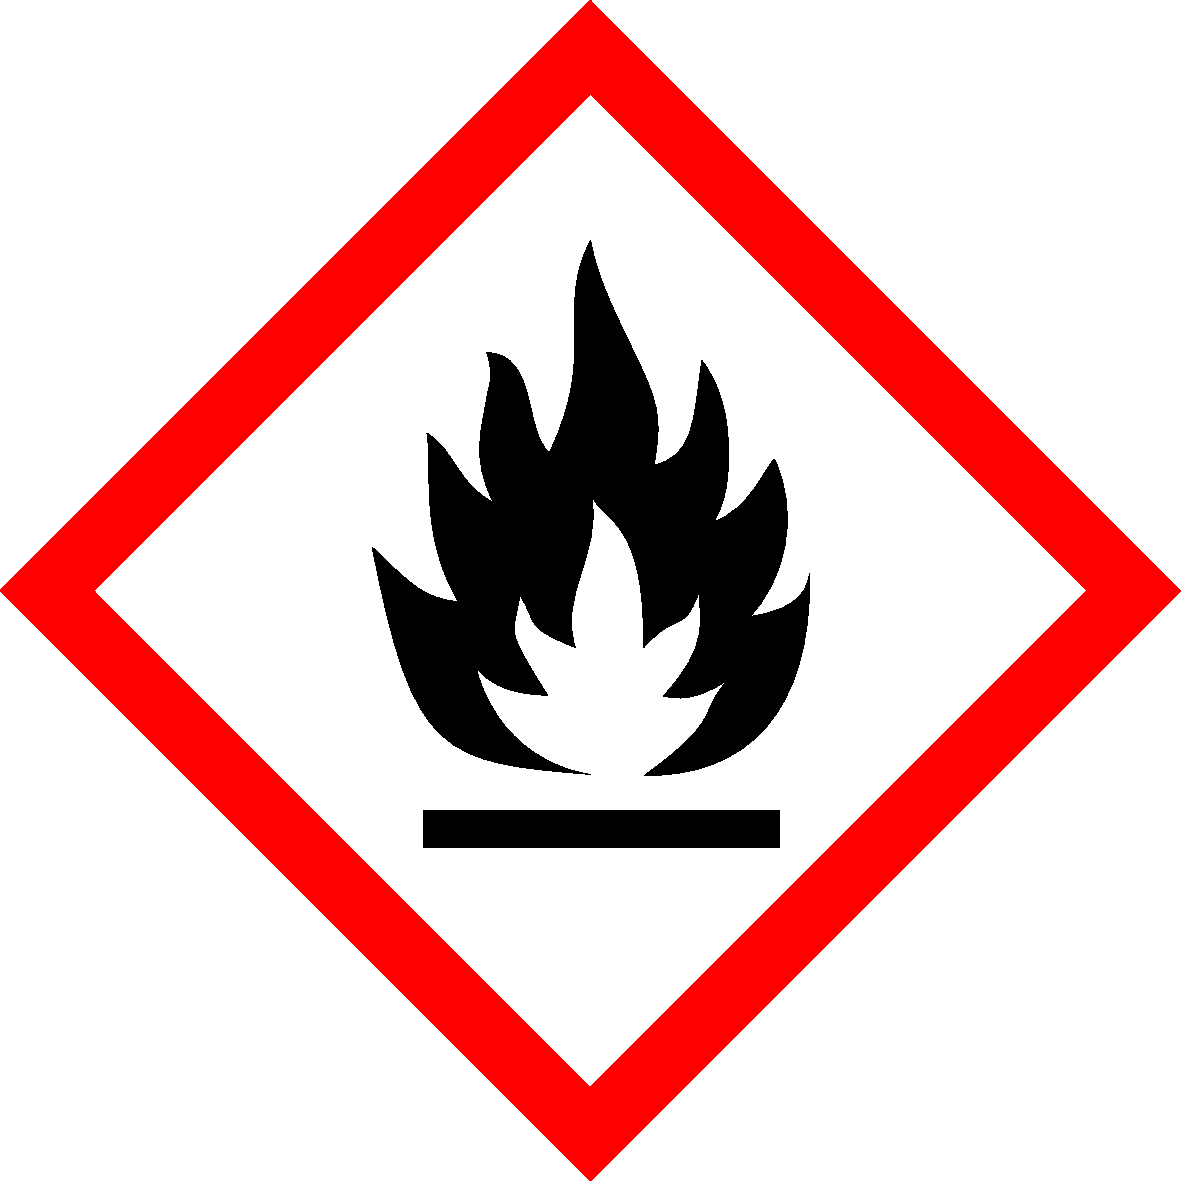
\includegraphics[height=24pt,valign=t]{pictos/flamm.pdf}
\includegraphics[height=24pt,valign=t]{pictos/exclam.pdf} & H225, H319 \newline P210, P241, P280, P303+P361+P353, P305+P351+P338, P501b
\\
\midrule
Rouge de méthyle, Solution\newline (269,3 g/mol) & 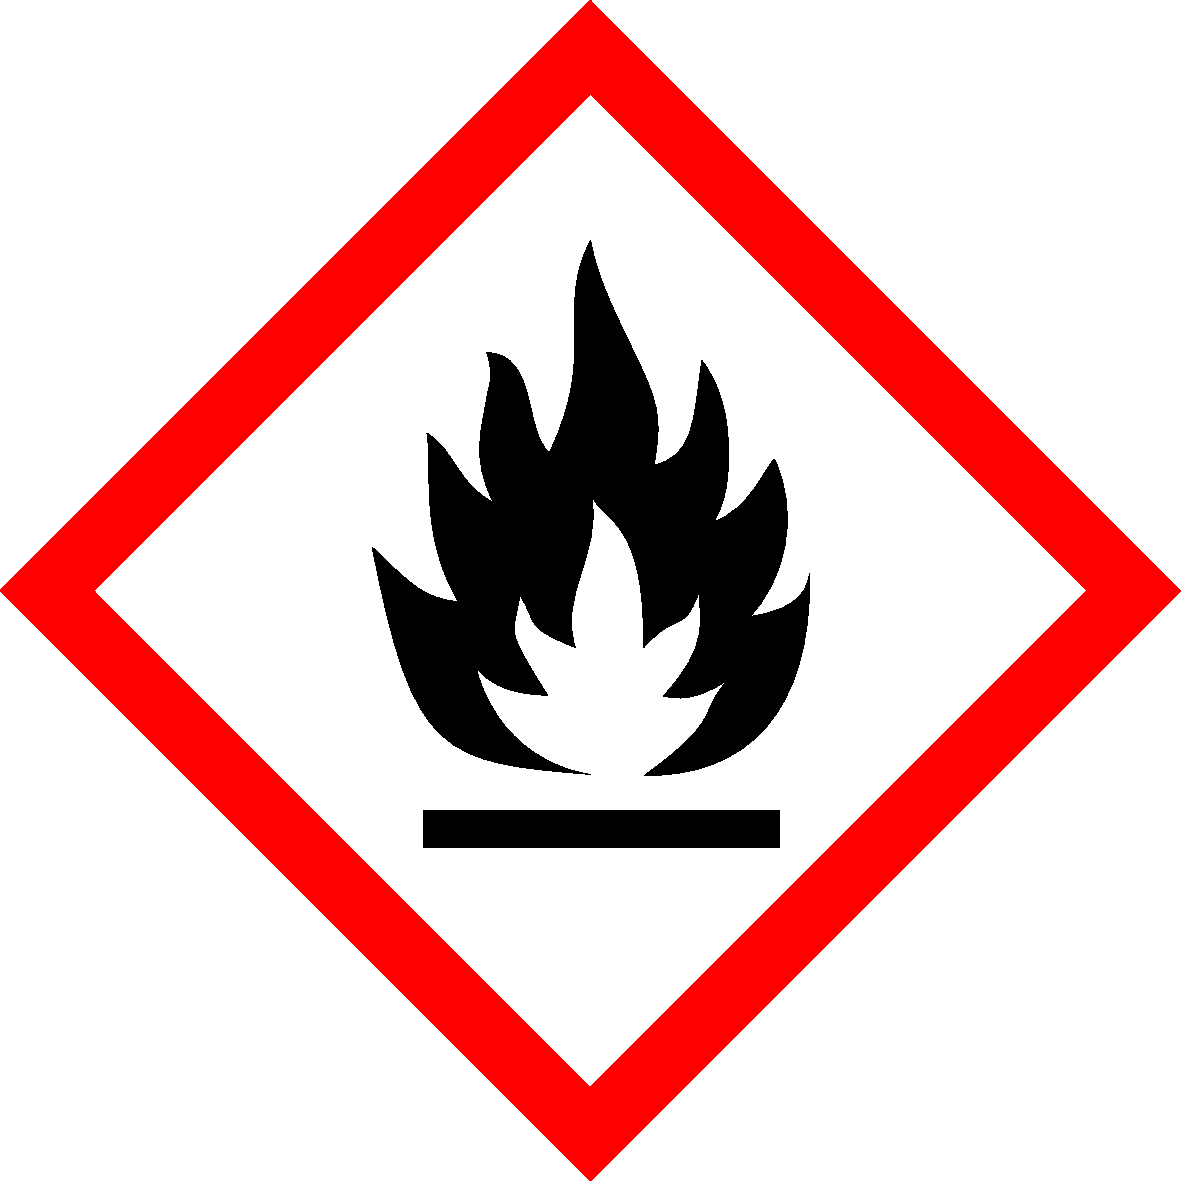
\includegraphics[height=24pt,valign=t]{pictos/flamm.pdf}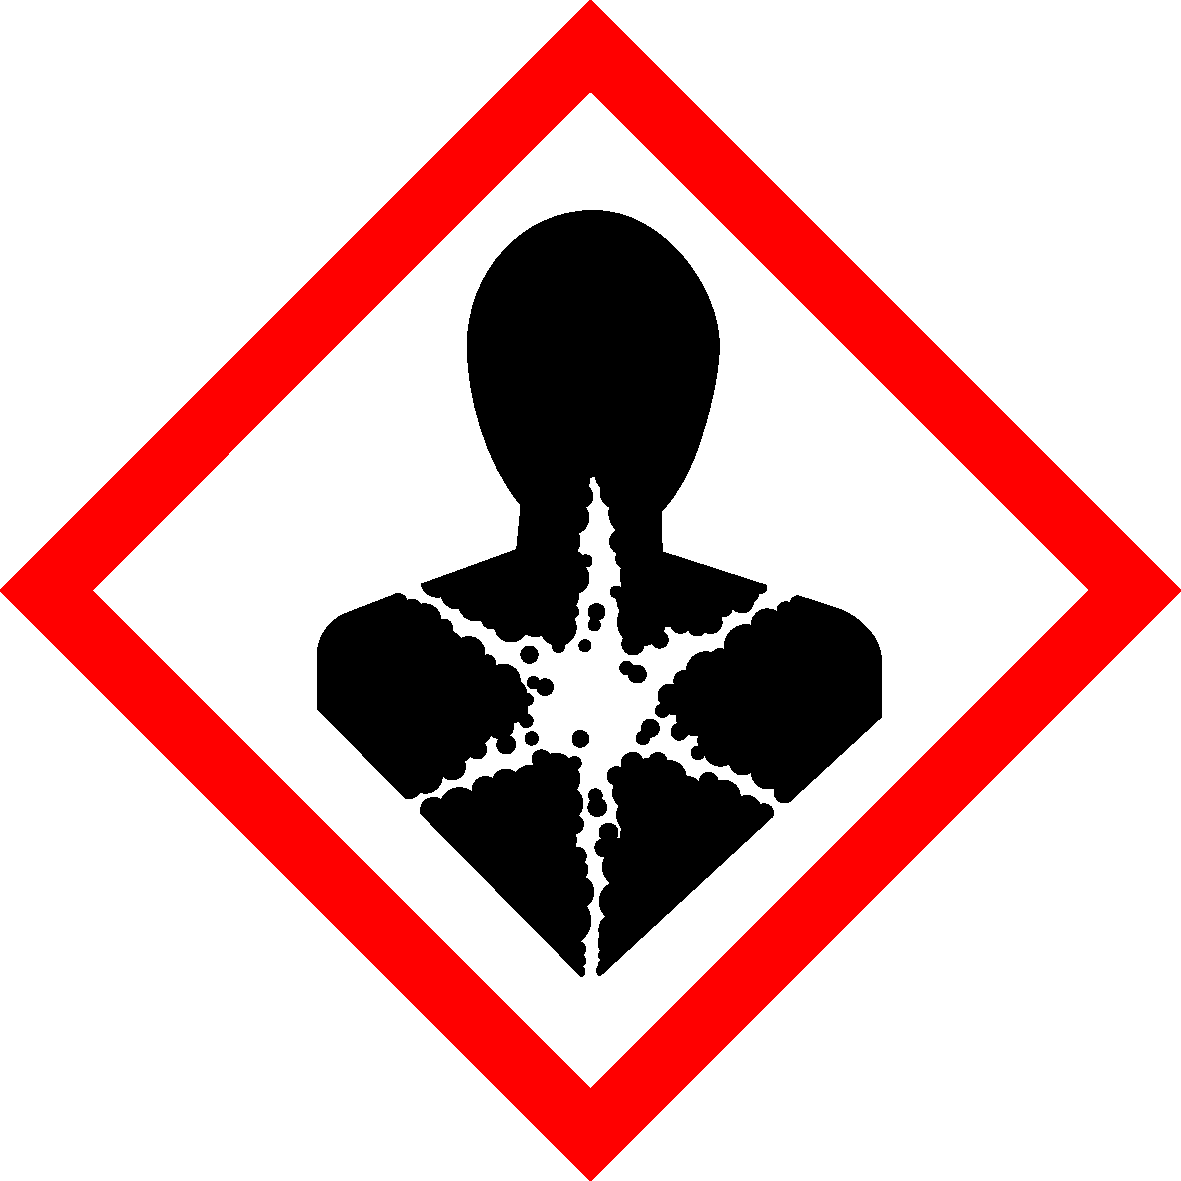
\includegraphics[height=24pt,valign=t]{pictos/cmr.pdf} 
\includegraphics[height=24pt,valign=t]{pictos/exclam.pdf} &  
H225, H319, H371\newline P210, P260, P280, P308 + P311, P337 + P313, P403 + P235\\
\midrule

\end{tabular}

\noindent\begin{tabular}{p{6.7cm}p{2cm}p{7cm}rrrrrrrrrr}
\midrule

Phenolphtaléine \newline (318,33 g/mol) &  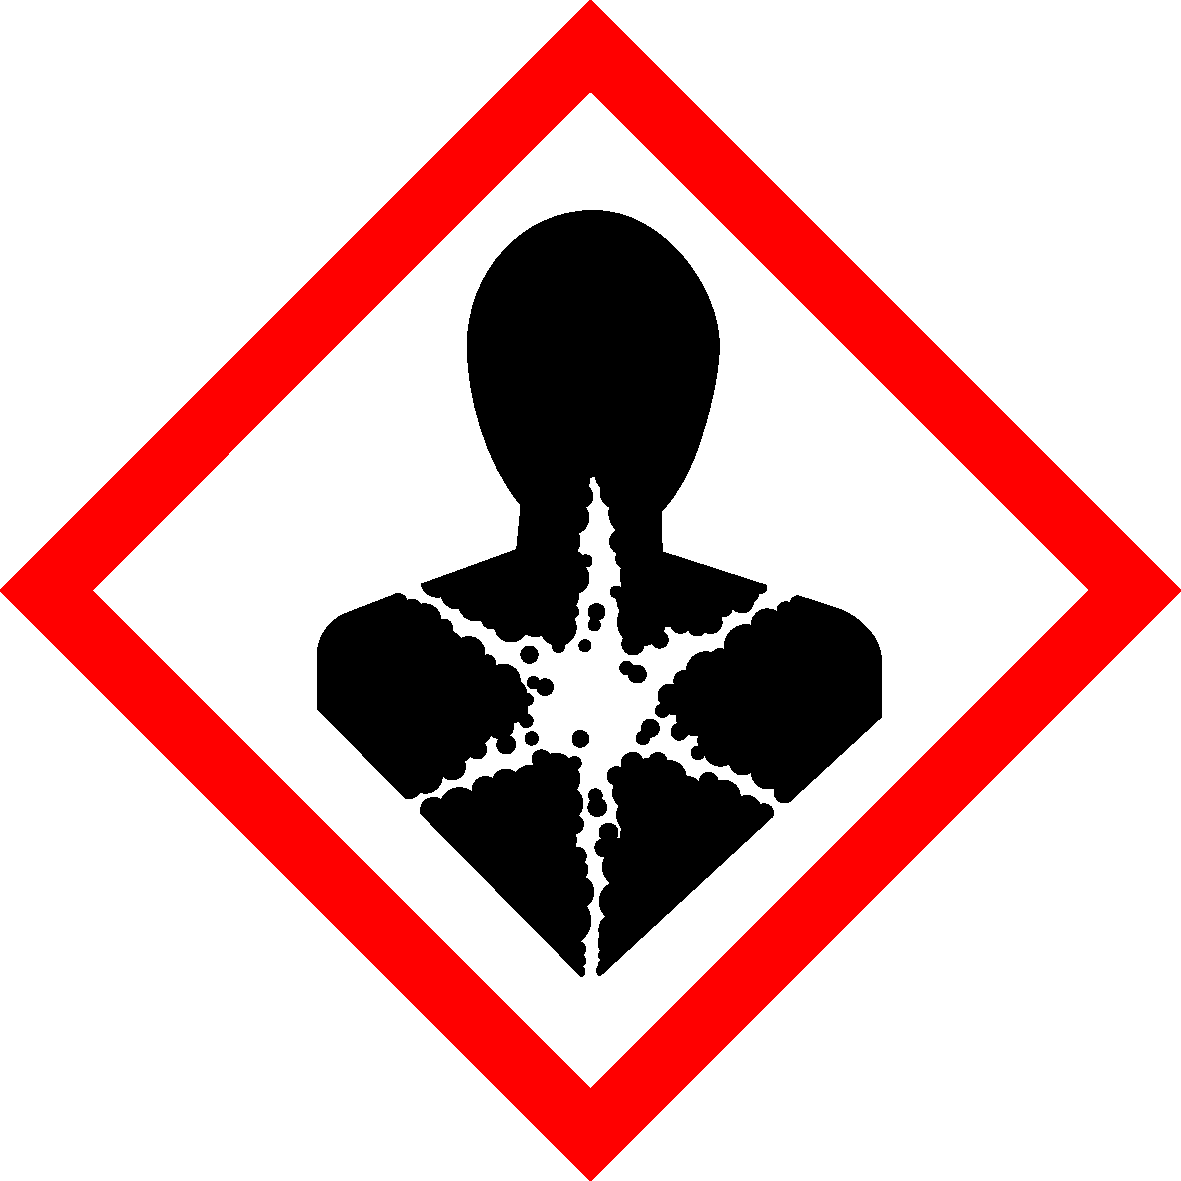
\includegraphics[height=24pt,valign=t]{pictos/cmr.pdf} & \\
\midrule

Acétate d'éthyle\newline (88,11 g/mol) & 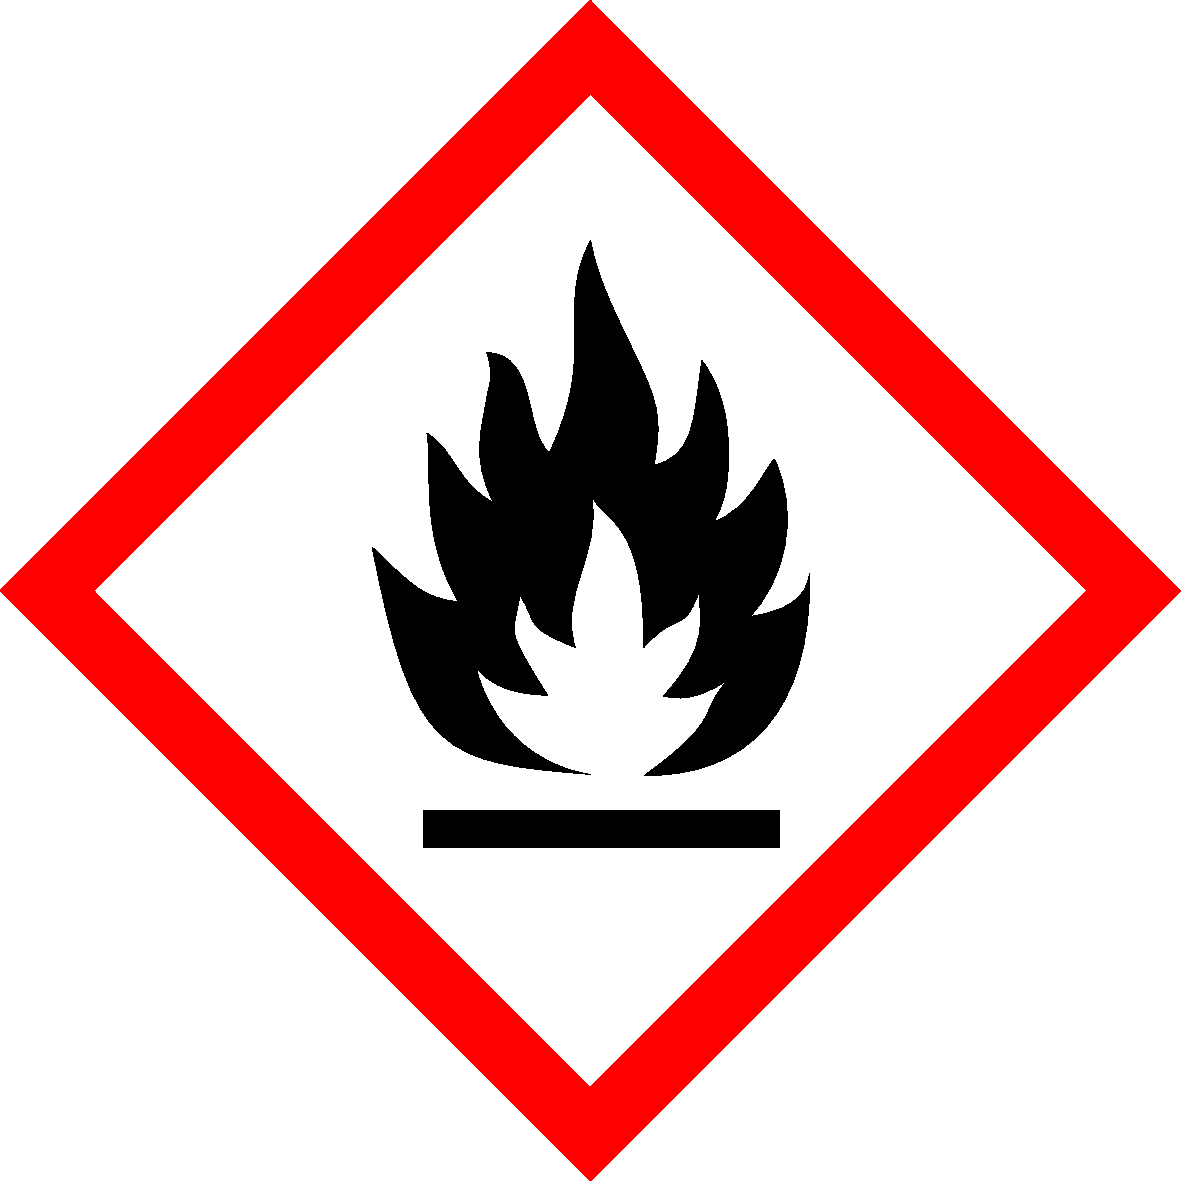
\includegraphics[height=24pt,valign=t]{pictos/flamm.pdf}
\includegraphics[height=24pt,valign=t]{pictos/exclam.pdf} &  
H225, H319, H336\newline P210, P305 + P351 + P338, P370 + P378, P403 + P235\\
\midrule
Cyclohexane \newline (84,16 g/mol) & 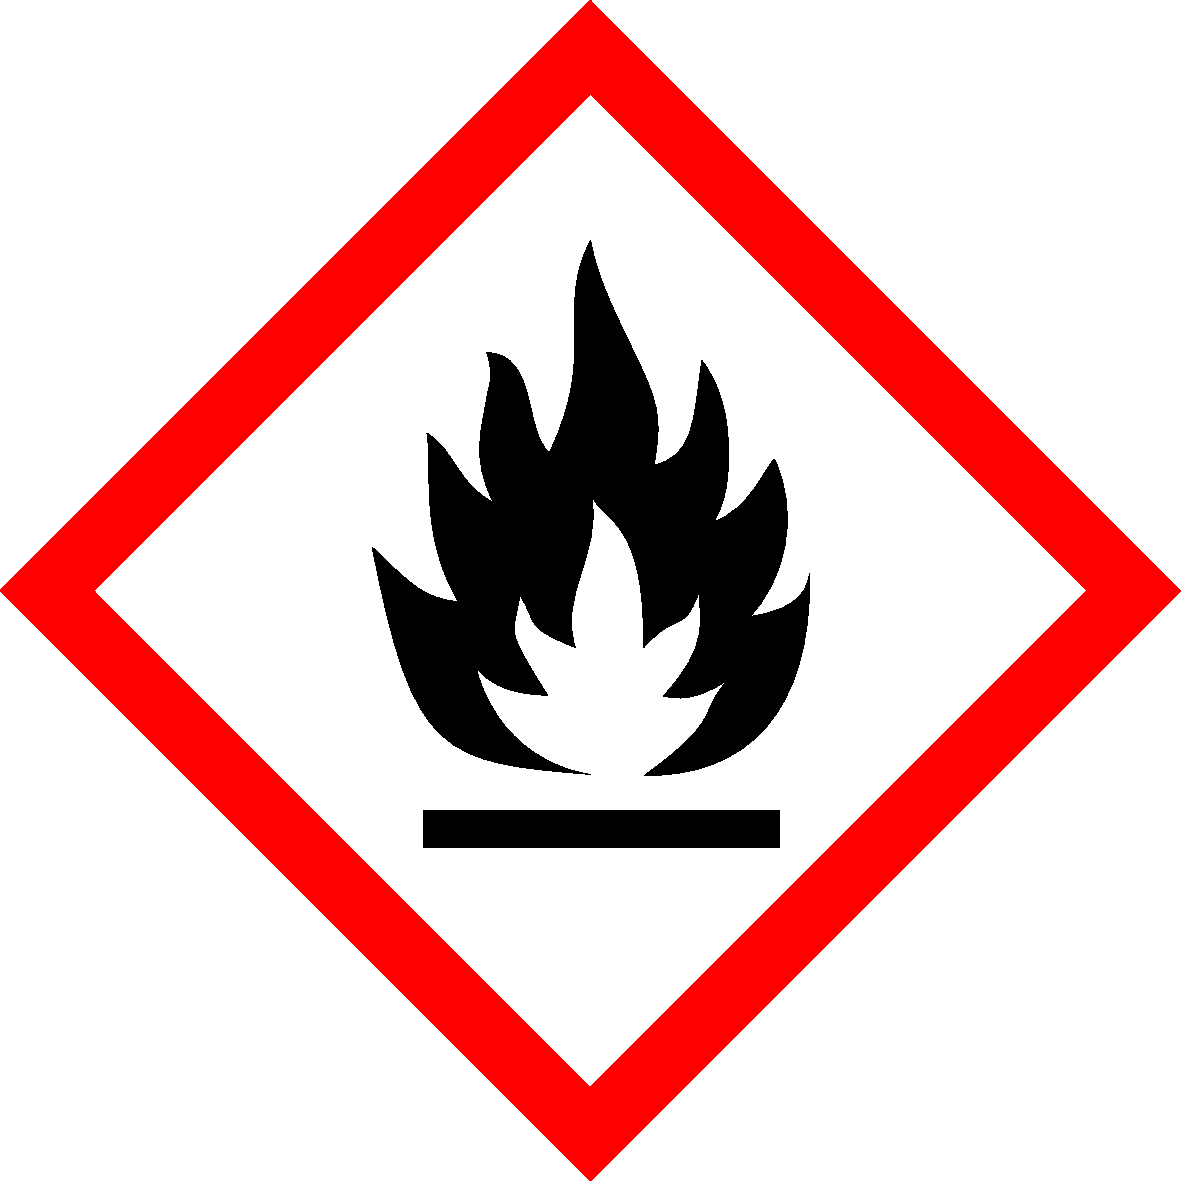
\includegraphics[height=24pt,valign=t]{pictos/flamm.pdf}
\includegraphics[height=24pt,valign=t]{pictos/exclam.pdf} 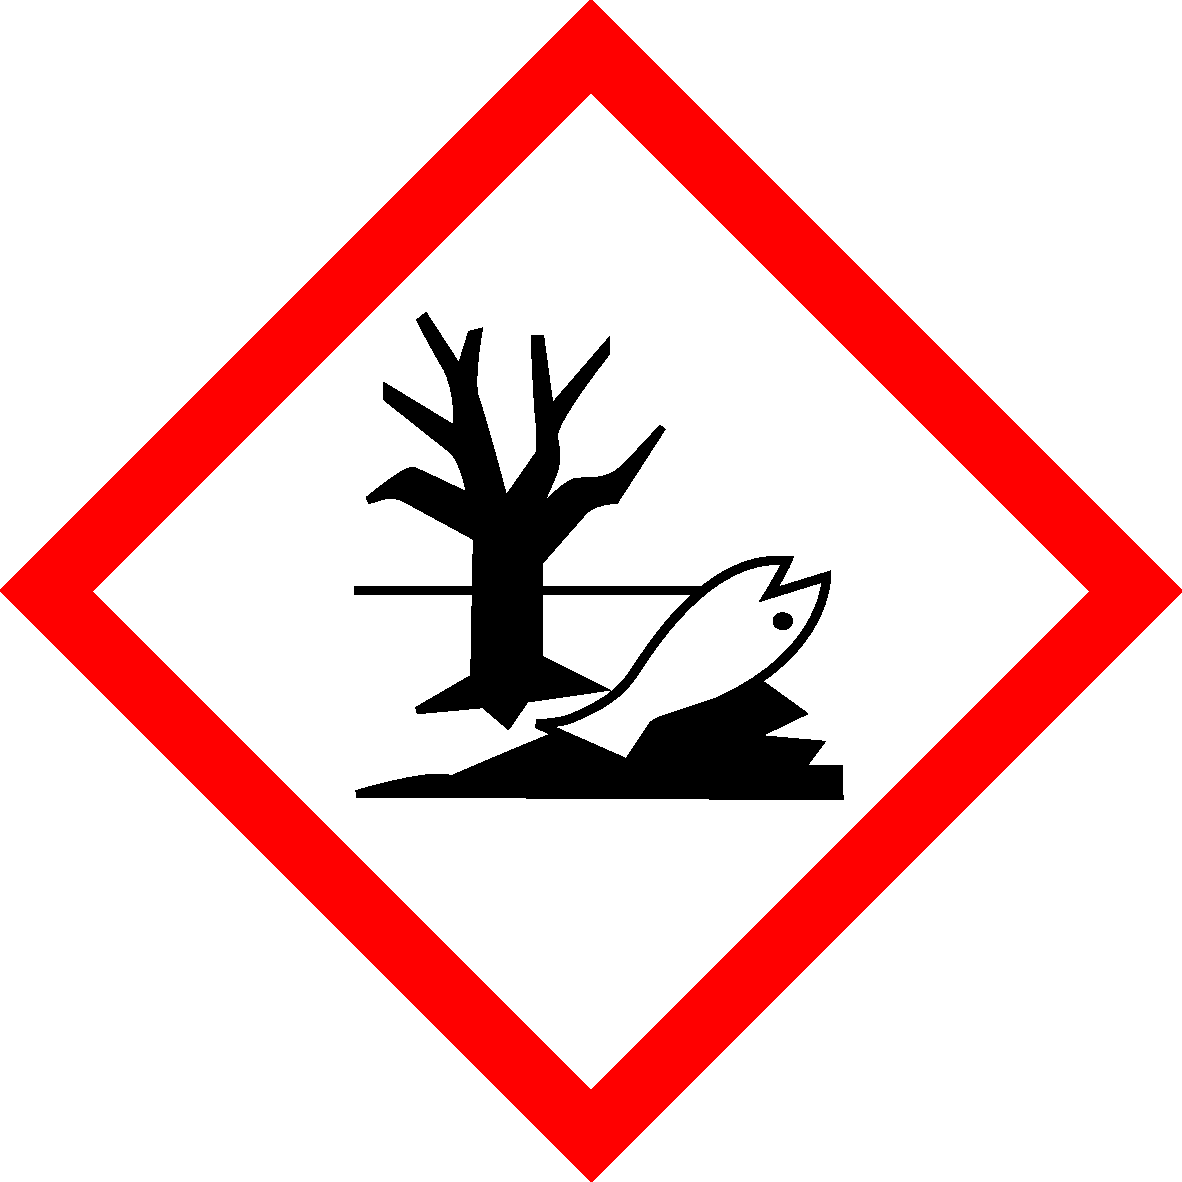
\includegraphics[height=24pt,valign=t]{pictos/envi.pdf} 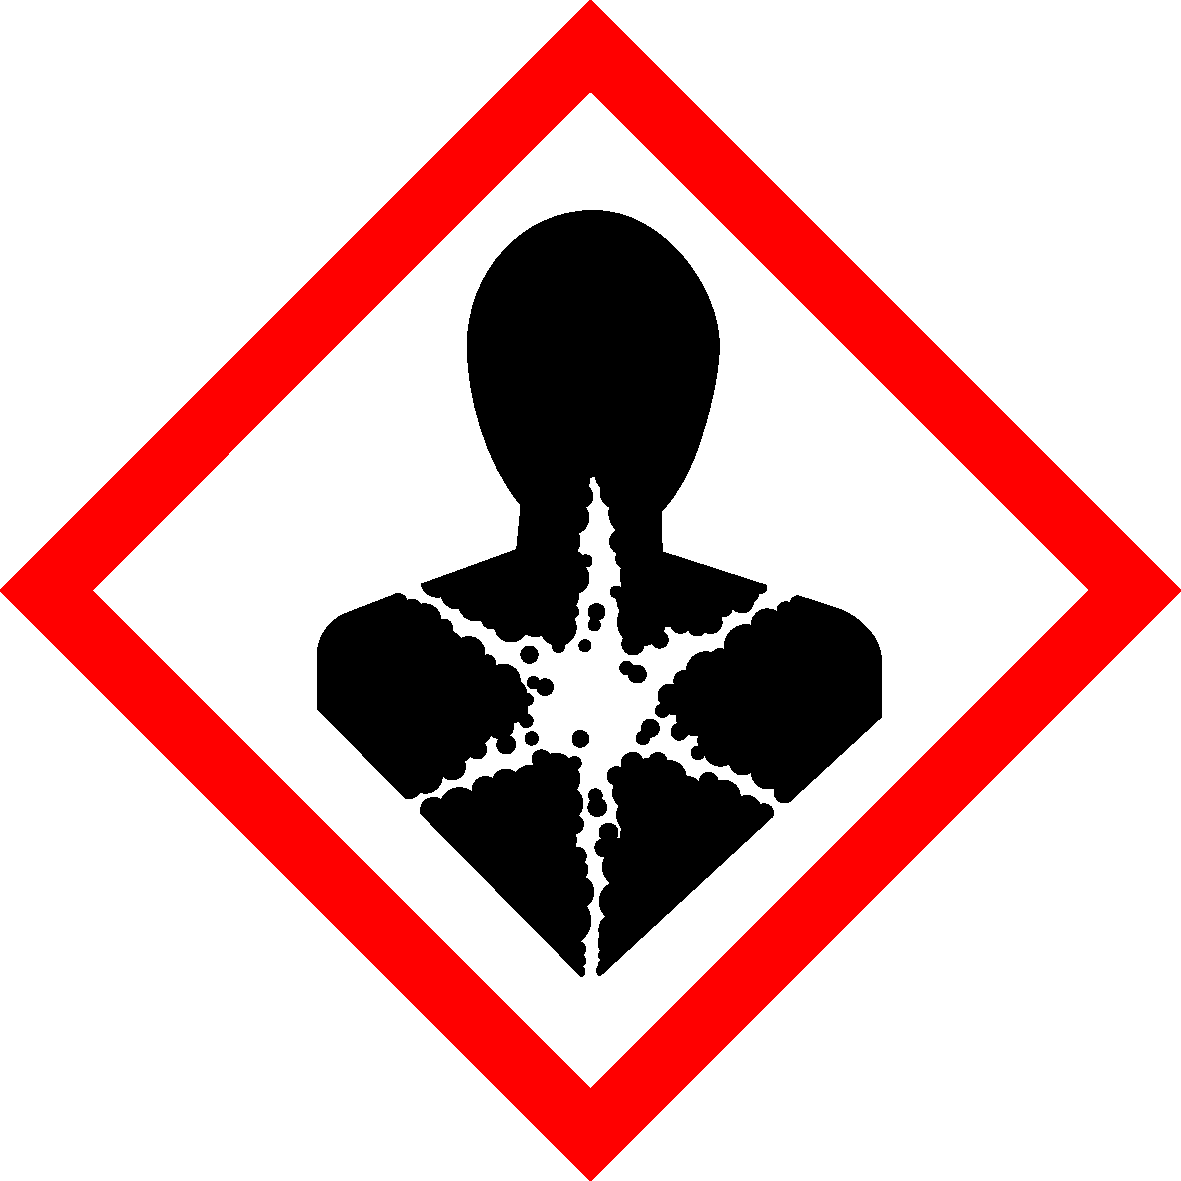
\includegraphics[height=24pt,valign=t]{pictos/cmr.pdf}   &  
H225, H304, H315, H336, H410 \newline P210, P233, P273, P301 + P310, P303 + P361 + P353, P331, P403 + P233 \\
\midrule
Ethanol, \newline (46,07 g/mol) & 
\includegraphics[height=24pt,valign=t]{pictos/exclam.pdf}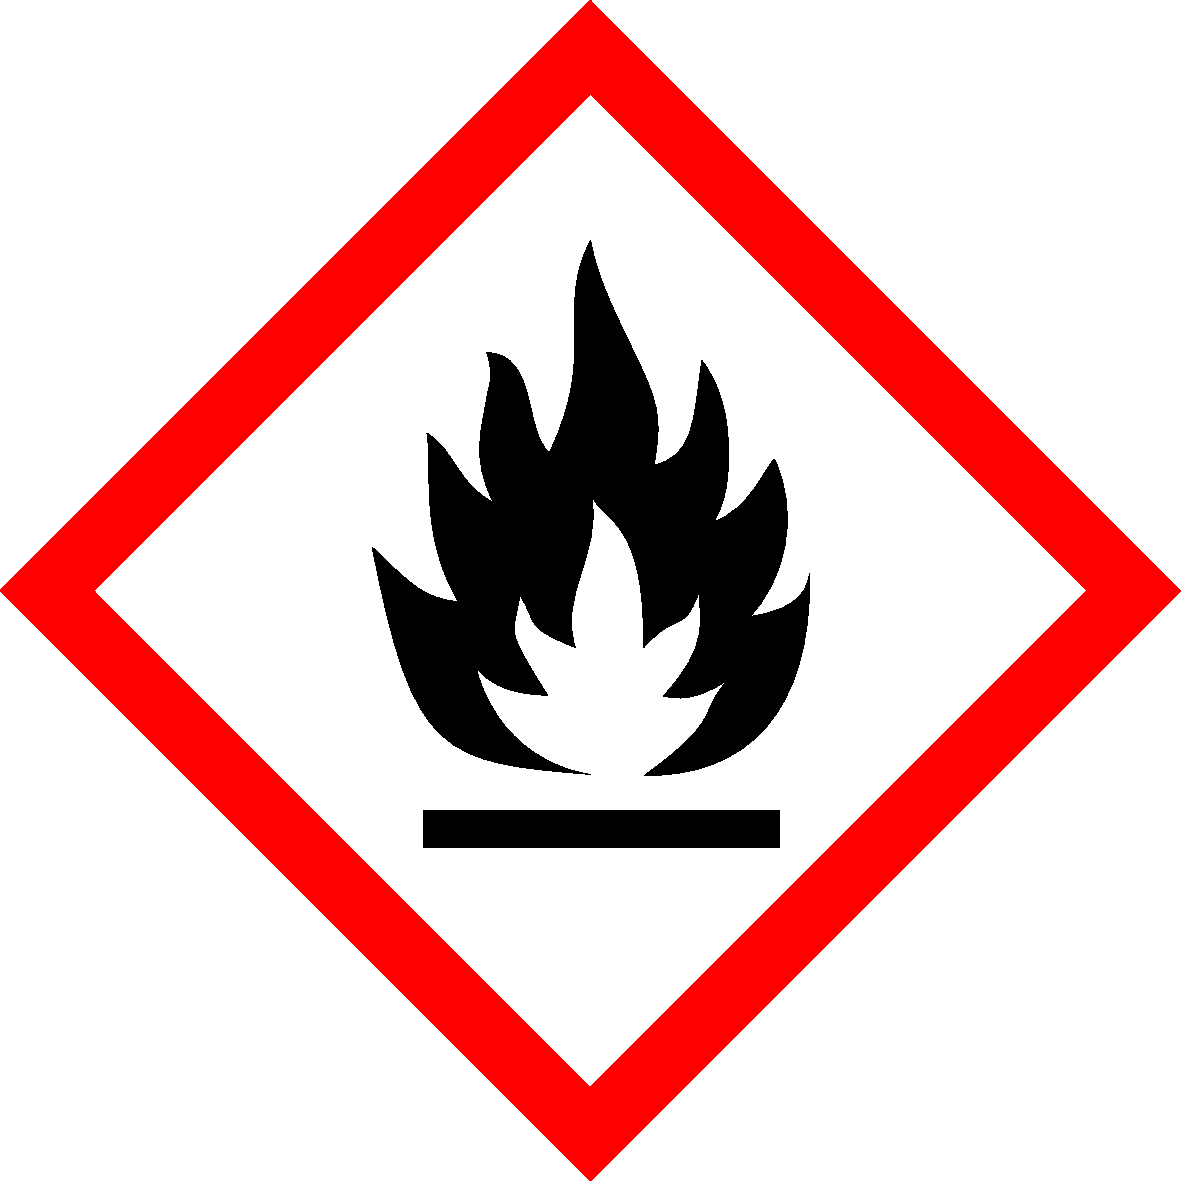
\includegraphics[height=24pt,valign=t]{pictos/flamm.pdf}  &  
H225, H319 \newline P210, P233, P240, P241, P242, P305 + P351 + P338, P403 + P233 \\
\midrule
Éther diéthylique \newline (74,12 g/mol) & 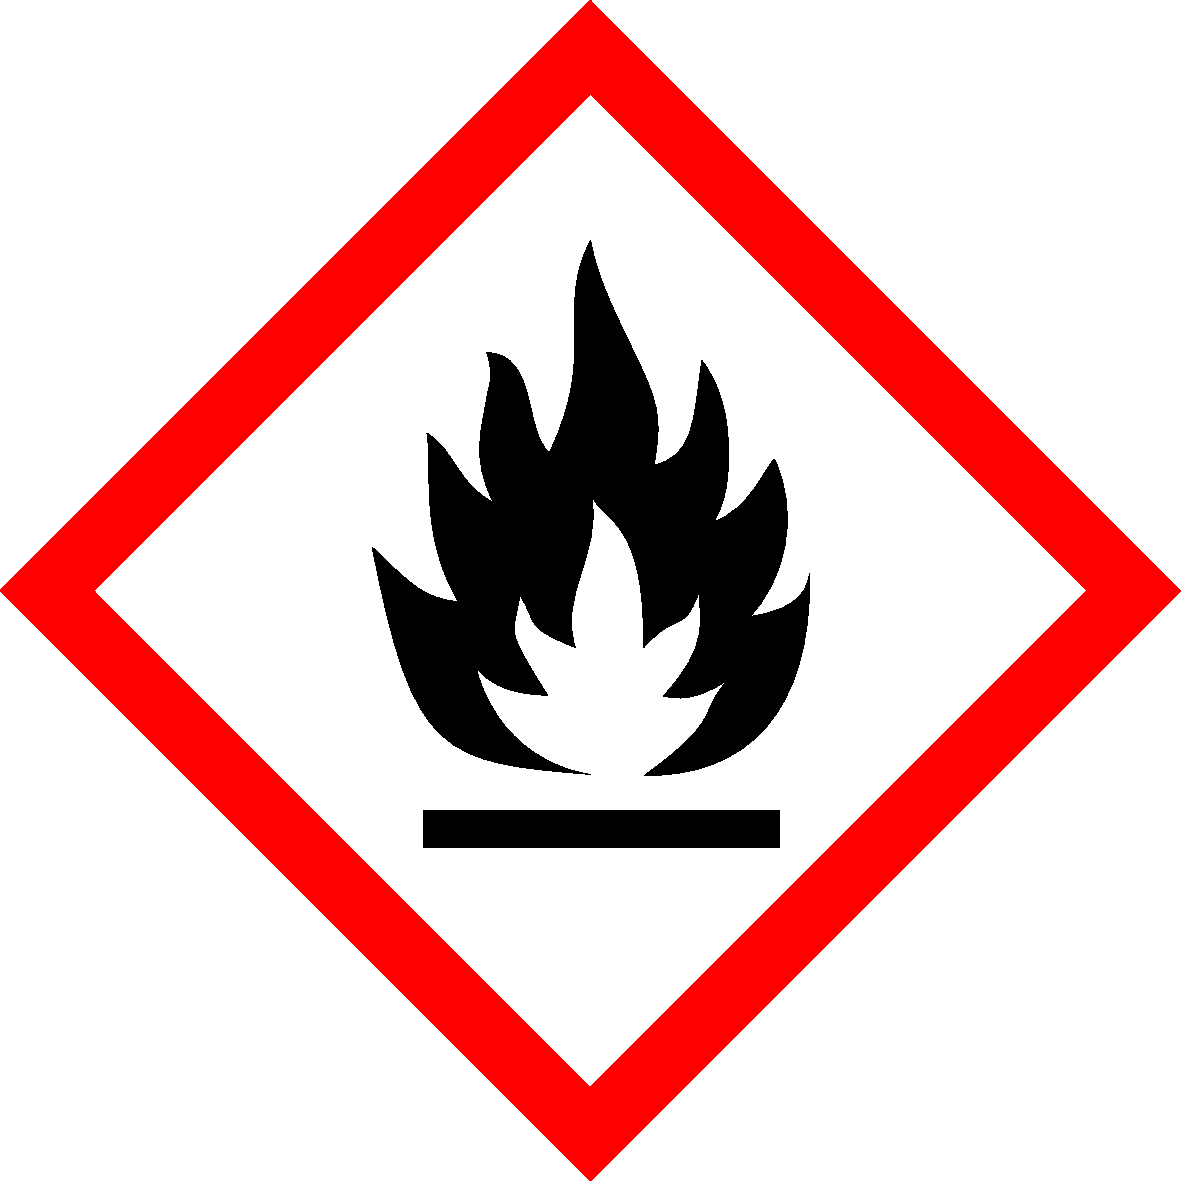
\includegraphics[height=24pt,valign=t]{pictos/flamm.pdf}
\includegraphics[height=24pt,valign=t]{pictos/exclam.pdf}  &  
H224 , H302 , H336 \newline P210 , P233 , P240 , P241 , P301 + P312, P403 + P233 \\
\midrule
\bottomrule
\end{tabular}



\end{document}
